%%%%%%%%%%%%%%%%%%%%%%%%%%%%%%  IEEEsample.tex  %%%%%%%%%%%%%%%%%%%%%%%%%%%%%%%
%%%%%%%%%%                                                        %%%%%%%%%%%%%
%%%%%%%%%%    More information: see the header of IEEEtran.sty    %%%%%%%%%%%%%
%%%%%%%%%%                                                        %%%%%%%%%%%%%
%%%%%%%%%%%%%%%%%%%%%%%%%%%%%%%%%%%%%%%%%%%%%%%%%%%%%%%%%%%%%%%%%%%%%%%%%%%%%%%
%
%\documentstyle[twocolumn]{IEEEtran}

%\documentclass[a4paper]{article}

% The amsmath and epsfig packages greatly simplify the process of adding
% equations and figures to the document, and thus their use is highly
% recommended.
% ------------

\documentclass[runningheads,a4paper]{llncs}


\usepackage{amsmath}
\usepackage{epsfig}
\usepackage{graphicx}
\usepackage{acronym}
\usepackage{array}
\usepackage{listings}
\usepackage[latin1]{inputenc}
\usepackage{amsmath}
\usepackage{amsfonts}
\usepackage{amssymb}
\usepackage{graphicx} 
\usepackage[latin1]{inputenc}
\usepackage{amsmath}
\usepackage{amsfonts}
\usepackage{amssymb}  
\usepackage{fancyhdr}
\usepackage{listings}
\usepackage{url}
\usepackage{float}

\usepackage{acronym}
\usepackage{caption}
\usepackage{subcaption}
\usepackage{setspace}
\usepackage{underlin}
\usepackage{algpseudocode}
\usepackage{algorithm}
\usepackage{amssymb}
\usepackage{booktabs}
\usepackage{makeidx} 
\usepackage{microtype} 


\newcommand{\HRule}{\rule{\linewidth}{0.5mm}}

\acrodef{fpga}[FPGA]{Field programmable gate array}
\acrodef{cpld}[CPLD]{complex programmable logic device}
\acrodef{asic}[ASIC]{application specific integrated circuits}
\acrodef{isa}[ISA]{instruction set architecture}
\acrodef{gpu}[GPU]{graphic processing unit}
\acrodef{fpu}[FPU]{floating processing unit}
\acrodef{hdl}[HDL]{hardware description language}
\acrodef{api}[API]{application programming interface}
\acrodef{ip}[IP]{intellectual property}
\acrodef{lut}[LUT]{lookup tables}
\acrodef{bram}[BRAM]{block RAM}
\acrodef{dsu}[DSU]{debug support unit}
\acrodef{alu}[ALU]{arithmetic logical unit}
\acrodef{cam}[CAM]{custom address memory}
\acrodef{hll}[HLL]{higher level languages}
\acrodef{cpu}[CPU]{central processing unit}
\acrodef{par}[PAR]{place and route}
\acrodef{ai}[AI]{artificial intelligence}
\acrodef{ipc}[IPC]{instruction per cycle}
\acrodef{fd}[FD]{finite difference}
\acrodef{ea}[EA]{evolutionary algorithms}
\acrodef{ann}[ANN]{artificial neural network}
\acrodef{svm}[SVM]{support vector machines}
\acrodef{veb}[VEB]{virtual embedded block}
\acrodef{mmu}[MMU]{Memory Management Unit}
\acrodef{cpld}[CPLD]{complex programmable logic device}
\acrodef{asic}[ASIC]{application specific integrated circuits}
\acrodef{isa}[ISA]{instruction set architecture}
\acrodef{gpu}[GPU]{graphic processing unit}
\acrodef{fpu}[FPU]{floating processing unit}
\acrodef{hdl}[HDL]{hardware description language}
\acrodef{api}[API]{application programming interface}
\acrodef{ip}[IP]{intellectual property}
\acrodef{lut}[LUT]{lookup tables}
\acrodef{bram}[BRAM]{block RAM}
\acrodef{dsu}[DSU]{debug support unit}
\acrodef{alu}[ALU]{arithmetic logical unit}
\acrodef{cam}[CAM]{custom address memory}
\acrodef{hll}[HLL]{higher level languages}
\acrodef{cpu}[CPU]{central processing unit}
\acrodef{par}[PAR]{place and route}
\acrodef{ai}[AI]{artificial intelligence}
\acrodef{ipc}[IPC]{instruction per cycle}
\acrodef{fd}[FD]{finite difference}
\acrodef{ea}[EA]{evolutionary algorithms}
\acrodef{ann}[ANN]{artificial neural network}
\acrodef{svm}[SVM]{support vector machines}
\acrodef{veb}[VEB]{virtual embedded block}
\acrodef{mmu}[MMU]{Memory Management Unit}
\acrodef{rmt}[RMT]{remapping table}
\acrodef{lnreg}[LNreg]{Line Number Register}
\acrodef{secrand}[SecRAND]{Security-Aware Random Replacement Algorithm}
\acrodef{aes}[AES]{Advanced Encryption System}
\acrodef{asi}[ASI]{Address space identifier}
\acrodef{fsm}[FSM]{Finite State Machines}
\acrodef{pca}[PCA]{Principal Component Analysis}
\acrodef{asip}[ASIP]{Application Specific Instruction Processor}
\acrodef{gp}[GP]{Gaussian Process}
\acrodef{gbsa}[GbSA]{Galaxy-based Search Algorithm}
\acrodef{aco}[ACO]{Ant Colony Optimization}
\acrodef{pso}[PSO]{Particle Swarm Optimization}
\acrodef{sa}[SA]{Simulated Annealing}
\acrodef{ga}[GA]{Genetic Algorithm}
\acrodef{iwdp}[IWDP]{Intelligent Water Drops}
\acrodef{hpc}[HPC]{High Performance Computing}
\acrodef{ib}[IB]{Investment Banking}
\acrodef{par}[PAR]{Place and Route}
\acrodef{agppso}[A-GP-PSO]{Adaptive Gaussian Process Particle Swarm Optimizer}
\acrodef{vpso}[VPSO]{Adaptive Velocity Particle Swarm Algorithm}
\acrodef{aes}[AES]{Advanced Encryption System}
\acrodef{cad}[CAD]{Computer Aided Design}
\acrodef{svm}[SVM]{Support Vector Machine}
\acrodef{alo}[MLO]{Machine Learning Optimizer}
\acrodef{rvm}[RVM]{Relevance Vector Machine}
\acrodef{rbf}[RBF]{Radial Basis Function}
\newcommand{\ra}[1]{\renewcommand{\arraystretch}{#1}}

\newcommand{\keywords}[1]{\par\addvspace\baselineskip
\noindent\keywordname\enspace\ignorespaces#1}

\pagestyle{headings}

\begin{document}

\mainmatter  % start of an individual contribution

\title{Parametric Optimization of Reconfigurable Designs using Machine Learning}

% a short form should be given in case it is too long for the running head
\titlerunning{Parametric Optimization with Machine Learning Optimizer}

% the name(s) of the author(s) follow(s) next
%
% NB: Chinese authors should write their first names(s) in front of
% their surnames. This ensures that the names appear correctly in
% the running heads and the author index.
%
\author{Maciej Kurek \and Tobias Becker \and Wayne Luk}
%
\authorrunning{M. Kurek, T. Becker and W. Luk}
% (feature abused for this document to repeat the title also on left hand pages)

% the affiliations are given next; don't give your e-mail address
% unless you accept that it will be published
\institute{Department of Computing, Imperial College London}

\toctitle{Lecture Notes in Computer Science}
\tocauthor{Authors' Instructions}
\maketitle


\begin{abstract}


This paper presents a novel technique that uses meta-heuristics and machine learning to automate the optimization of design parameters for reconfigurable designs. Traditionally, such an optimization involves manual application analysis as well as model and parameter space exploration tool creation. We develop a \ac{alo} to automate this process. From a number of benchmark executions, we automatically derive the characteristics of the parameter space and create a surrogate fitness function through regression and classification. Based on this surrogate model, design parameters are optimized with meta-heuristics. We evaluate our approach using two case studies, showing that the number of benchmark evaluations can be reduced by up to 85\% compared to previously performed manual optimization.


\keywords{optimization, surrogate modeling, PSO, GP, SVM, FPGA}

\end{abstract}

\section{Introduction}

\acp{fpga} allow designs that are customized to the requirement of the application. Reconfiguration is an additional benefit which allows the designer to modify designs at run time, potentially increasing performance and efficiency. Unfortunately, the optimization of reconfigurable designs often requires substantial effort from designers who have to analyze the application, create models and benchmarks and subsequently use them to optimize the design. This process often involves adjusting multiple design parameters such as numerical precision, degree of pipelining or number of cores. One could proceed with automated optimization based on an exhaustive search through design parameters which are derived from application benchmarks; however, this is unrealistic since benchmark evaluations involve bitstream generation and code execution which often takes hours of compute time.


It has been shown useful to construct surrogate models of fitness functions representing design quality for computationally expensive optimization problems in various fields \cite{1041556,surrogateModel,Su:2008:GPA:1494644.1494688,5194095,LeThi2002258}. As these models are orders of magnitude faster to evaluate than the actual fitness function, they can substantially accelerate optimization thus allowing for an automated approach. This is the motivation behind our development of the \ac{alo} tool which we apply to the problem of reconfigurable designs parameter optimization. In \cite{fpt2012MLO} we present initial concepts on optimizing parameter configuration of reconfigurable designs using surrogate models. We now present the formalism and experimental evaluation for our approach. The contributions of this paper are: 

\vspace{-0.5em}

\begin{list}{$\bullet$}{\itemsep 0.5ex}

\item A mathematical characterization of the parameter space for reconfigurable designs as well as a definition of a fitness function based on application benchmarks (Section \ref{design}).

\item Generic surrogate models to approximate the fitness function using regression and classification. We combine surrogate models with meta-heuristics to provide a new \ac{alo} algorithm for automated optimization of reconfigurable designs (Section \ref{surrogatemodels}).

\item An evaluation of our \ac{alo} approach in two case studies: (a) execution time of a run-time reconfigurable software-defined radio with varied degree of parallelism, and (b) and a previously used \cite{fpt2012MLO} throughput of a quadrature based financial application with varied precision (Section \ref{evaluation}).
\end{list}




\section{Background}


When developing reconfigurable applications, designers are often confronted with a very large parameter space. As a result the parameter space exploration can take an immense amount of time. A number of researchers approach the problem of high-cost fitness functions and large design spaces in various fields \cite{1041556,surrogateModel,Su:2008:GPA:1494644.1494688,5194095,LeThi2002258} by having fitness functions combined with fast-to-compute surrogate models provided by a \ac{gp} for decreasing evaluation time. However most current surrogate models only consist of a regressor and do not take into account possible invalid configurations within the design space. Furthermore, all of them are evaluated using artificial benchmarks spanned by continuous $\mathbb{R}^n$ spaces, while parameter spaces for reconfigurable applications usually also involve discrete dimensions (e.g. number of cores). Surrogate models approximating fitness functions by substituting lengthy evaluations with estimations based on closeness in a design space have been investigated in reconfigurable computing \cite{Pilato2008}. The work covers surrogate models for circuit synthesis from \ac{hll}, rather than parameter optimization.


%\vspace{-1em}

%\subsection{Gaussian Process Regression}

\ac{gp} is a machine learning technology based on strict theoretical fundamentals and Bayesian theory \cite{Seeger04gaussianprocesses,Rasmussen06gaussianprocesses}. \ac{gp} does not require a predefined structure, can approximate arbitrary function landscapes including discontinuities, and includes a theoretical framework for obtaining the optimum hyper-parameters \cite{5194095}. An advantage of \ac{gp} is that it provides a predictive distribution, not a point estimate.

 %can have meaningful hyper-parameters,%

A Gaussian process is a collection of random variables, any finite set of which have a joint Gaussian distribution. A Gaussian process is completely specified by its mean function $m(\mathbf{x})$ and the covariance (kernel) function $k(\mathbf{x},\mathbf{x'})$:

%\vspace{-1em}


\begin{align} 
\hat{f}(\mathbf{x}) \sim \mathcal{G}\mathcal{P}(m(\mathbf{x}),k(\mathbf{x},\mathbf{x'}))
\end{align}

%\vspace{-0.5em}

The $k(\mathbf{x},\mathbf{x'})$ expresses the covariance between pairs of random variables, and in regression analysis it expresses the relation between input-output pairs. This is based on a training set $\mathcal{D}$ of $n$ observations, $\mathcal{D}={(\mathbf{x}_i,y_{i}) | i = 1, ... n} $, where $\mathbf{x}$ denotes an input vector, $y$ denotes a scalar output. The column vector inputs for all $n$ cases are aggregated in the $D \times n$ design matrix $X$, and the outputs are collected in the vector $\mathbf{y}$. The goal of Bayesian forecasting is to compute the distribution $p(\hat{f}|\mathbf{x_*},\mathbf{y},X)$ of the function $\hat{f}$ at unseen input $\mathbf{x_{*}}$ given a set of training points $\mathcal{D}$. Using Bayes rule, the predictive posterior for the Gaussian process $\hat{f}$ and the predicted scalar outputs $\hat{f}(\mathbf{x_*})=y_*$ can be obtained.

% By conditioning on the observed targets in the training set, the predictive distribution is Gaussian.

%\vspace{-1em}


%\subsection{Support Vector Machines Classification}

\ac{svm} is a maximum margin classifier, which constructs a hyperplane used for classification (or regression) \cite{Bishop:2006:PRM:1162264}. \acp{svm} use kernel functions $k(\mathbf{x},\mathbf{x'})$ to transform the original feature space to a different space where a linear model is used for classification. \acp{svm} are a class of decision machines and so do not provide posterior probabilities. There is a training set $\mathcal{D}$ of $n$ observations, $\mathcal{D}={(\mathbf{x}_i,t_{i}) | i = 1, ... n} $, where $\mathbf{x}$ denotes an input vector, $t$ denotes a target value. The column vector inputs for all $n$ cases are aggregated in the $D \times n$ design matrix $X$, and the targets in the vector $\mathbf{t}$. The goal is to classify an unseen input $\mathbf{x_{*}}$ based on $X$ and $\mathbf{t}$ by computing a decision boundary. 

%\begin{align} 
%f(x) = w^{T} \phi(x) + \beta
%\end{align}

%\vspace{-1em}


%\subsection{Particle Swarm Algorithm (PSO)}
%with inertia governing its movement
\ac{pso} is a population-based meta-heuristic based on the simulation of the social behavior of birds within a flock \cite{VanDenBergh:2002:APS:935867}. The algorithm starts by randomly initializing $N$ particles where each individual is a point in the $\mathcal{X} = \mathbb{R} \times ... \times \mathbb{R}$ search space. The population is updated in an iterative manner where each particle is displaced based on its velocity $v_{id}$. The criteria for termination of the \ac{pso} algorithm can vary, and usually are determined by a time budget. The $x_{id}$ represents the $d$th coordinate of particle $i$ from the set $X_*$ of $N$ particles, where particle is a point within $\mathcal{X}$. In the most basic form of \ac{pso} Eq. \ref{eq:pso1}-\ref{eq:pso2} govern movement of particles. $r_1 \sim U(0,1)$ and $r_2 \sim U(0,1)$ are two independent uniformly distributed random numbers, $c_1$ and $c_2$ are acceleration coefficients and $p_{gd}$ and $p_{id}$ are $d$th coordinates of the global best and personal best positions. $p_{gd}$ is updated when a new global best fitness is found and $p_{id}$ is updated when a particle improves over its best fitness.

%\vspace{-1.5em}


\begin{align} 
\label{eq:pso1}
v_{id}=v_{id}+c_{1}r_{1}(p_{id}-x_{id}) + c_{2}r_{2}(p_{gd}-x_{id})
\end{align}

%\vspace{-2.5em}


\begin{align} 
\label{eq:pso2}
x_{id}=x_{id}+v_{id} 
\end{align}

%\vspace{-1.9em}

\section{Optimization Approach} 
\label{design}
%y fitness function of a heterogeneous application we understand fitness provided by execution of the applications benchmark.
%The challenge we address is encapsulation of reconfigurable designs $\mathcal{X}$ to provide an environment suitable for meta-heuristic to minimize benchmark evaluations. 
% If the optimizer fails to deliver optimal value, we have to increase its time and resource budget or re-design the application.

Traditionally, optimization of reconfigurable applications is carried out by building benchmarks and relevant tools, and the associated analytical models \cite{Anson2012Quad,Becker:2009:PDR:1530588.1530595}. This involves the following steps:

%\vspace{-0.5em}

\begin{enumerate}\addtolength{\itemsep}{-0.1\baselineskip}  
\item Build application and a benchmark returning design quality metrics.
\item Specify search space boundaries and optimization goal.
\item Create analytical models for the design.
\item Create tools to explore the parameter space.
\item Use the tools to find optimal configurations, guided by the models in step 3.
\item If result is not satisfactory, redesign.
\end{enumerate}

%\vspace{-0.5em}

In our approach the user supplies a benchmark along with constraints and goals, and the MLO automatically carries out the optimization (Algorithm \ref{ourmlo}). Our approach consists of the following steps:

\begin{enumerate}\addtolength{\itemsep}{-0.1\baselineskip}  
\item Build application and benchmark returning design quality metrics.
\item Specify search space boundaries and optimization goal.
\item Automatically optimize design with \ac{alo}.
\item If result is not satisfactory, redesign or revised time budget and search space.

\end{enumerate}

Our idea of surrogate modeling is illustrated in Fig.~\ref{fig:ouridea}. The \ac{alo} algorithm explores the parameter space by evaluating different benchmark configurations as presented in the left figure. The results obtained during evaluations are used to build a surrogate model which provides a regression of the fitness function and identifies invalid regions of the parameter space. A meta-heuristic (currently \ac{pso}) guides the exploration of the parameter space using the surrogate model. 

%Our steps 1, 2 and 4 correspond to traditional steps 1, 2 and 6. Therefore our approach is faster than the traditional
%approach if the time taken during our step 3 is shorter than the total time taken for steps 3, 4 and 5 of the traditional approach. Our approach will get faster the less time individual steps take. 

%We contrast two approaches in Fig.~\ref{fig:ouridea}.

  \begin{figure*}
     \centering
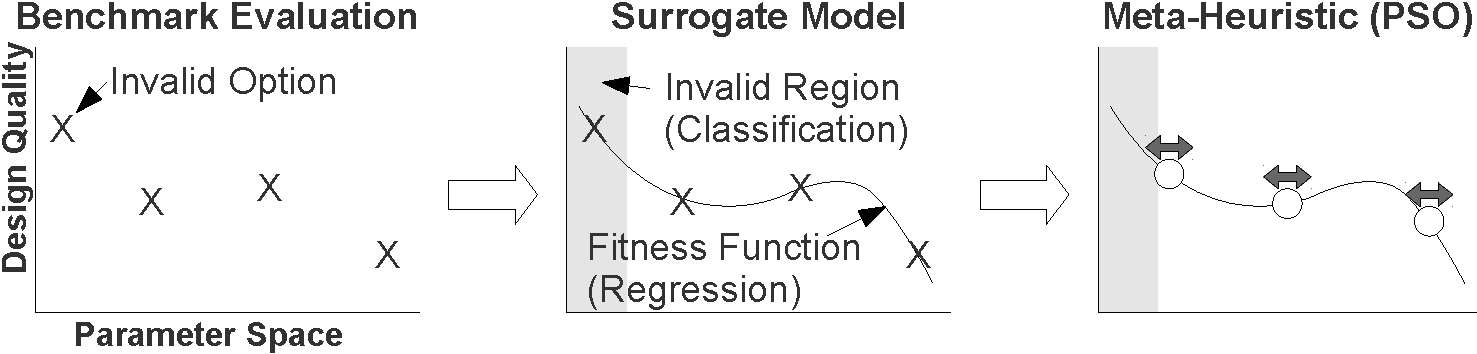
\includegraphics[width=1.0\textwidth]{./figs/surrogate_tobias.pdf}
        \caption{Benchmark evaluations, surrogate model and model guided search.}     
           \label{fig:ouridea}
  \end{figure*}
 
%We use meta-heuristics to explore parameter space. The challenge with applying meta-heuristics to reconfigurable design parameter optimization is related to high cost of fitness function evaluations (application benchmark evaluations). Our proposed optimization approach has three new aspects that counter this problem. We define a mathematical description of reconfigurable designs parameter space and provide a formal definition of the fitness function based on application benchmarks and the parameter space (Section \ref{designspace} and \ref{fitfunction})). By doing so we provide an environment suitable for meta-heuristic optimization. Using the defined parameter space and fitness function we build a surrogate model of application fitness function (Section \ref{surrogatemodels}) and we use it to define the new surrogate model aided meta-heuristic \ac{alo} (Section \ref{aloalgo}). Finally we explain how to determine \ac{alo} termination criteria depending on user goals (Section \ref{term}). 
%\vspace*{-2.5em}

\subsection{Parameter Space} 
\label{designspace}

The parameter space $\mathcal{X}$ of a reconfigurable design is spanned by discrete and continuous parameters determining both the architecture and physical settings of \ac{fpga} designs. A vector $\mathbf{x}$ represents a parameter configuration within the parameter space $\mathcal{X} = \mathcal{X}_1 \times ... \times \mathcal{X}_D $ such that any $\mathcal{X}_{d} \subseteq \mathbb{R}$. If $\mathcal{X}_{d} \subseteq \mathbb{Z}$, its discretization level is independent of other dimensions. $\mathcal{X}_{d}$ can be bounded with upper and lower limits $U_d,L_d$ such that for all $x_{d}$, $L_d \leq x_{id} \leq U_d$. An example of a continuous parameter is core frequency and an example of a discrete parameter is the number of compute cores. For all discrete dimensions the step size, which we define as smallest distance between any two $x_{id}$'s, can vary. We might only be able to increase memory width in 16 bits increments. 

%rember that the parameter space does not have to be uniform as well! not incldued yet

A discrete parameter space has important implications on the \ac{pso} algorithm, as the equations governing movements of particles Eq. \ref{eq:pso1}-\ref{eq:pso2} are defined for a continuous $\mathbb{R}^{n}$ space. In Eq. \ref{eq:pso1} both $r_{1}$ and $r_2$ are random real numbers, which means that the resulting velocity component used to update position $\mathbf{x}$ cannot be used if $x_d$ is discrete. To discretize the position value of a particle after its movement, we round its value and randomize its rounding error (dithering) presented in Eq. \ref{eq:dithering}. By using dithering instead of truncation \ac{pso} particles maintain their velocity component which results in a more thorough exploration.



%A discrete parameter space has important implications on the \ac{pso} algorithm, as the equations governing movements of particles Eq. \ref{eq:pso1}-\ref{eq:pso2} are defined for a continuous $\mathbb{R}^{n}$ space. In Eq. \ref{eq:pso1} both $r_{1}$ and $r_2$ are random real numbers, which means that the resulting velocity component used to update position $x$ cannot be used if $x_d$ is discrete. To discretize the position value of a particle after its movement, we round its value and randomize its rounding error (dithering). By using random rounding instead of truncation we allow \ac{pso} particles to maintain their velocity component which will result in a more thorough exploration. 

% We draw a uniformly distributed random number, and apply either floor or ceil functions depending on the value of sampled random number. 

%\vspace{-1.5em}

\begin{align} 
\label{eq:dithering}
x_{di} = 
\begin{cases}
\lfloor x_{id} \rfloor &  U(0,step size) < (x_{di}\mod{stepsize}\enspace)\\
\lceil x_{id} \rceil & U(0,step size) \ge (x_{di}\mod{stepsize}\enspace)\\
\end{cases}
\end{align}

%\vspace{-2em}

 \subsection{Fitness Function}
\label{fitfunction}

%, 

Given a parameter setting $\mathbf{x}$, the benchmark $b(\mathbf{x})$ returns a fitness metric which constitutes two values: $y$, the scalar metric of fitness and $t$, the exit code of the application. Execution time and power consumption are examples of fitness measures. There are be many possible exit codes $t$, with 0 indicating valid $\mathbf{x}$'s. The designer can choose to extend the benchmark to return additional exit codes depending on the failure cause, such as configurations producing inaccurate results or failing to build. 

We distinguish three different types of exit codes. The first type is exit code 0 indicating a valid design. The second type of exit codes indicate configurations that produce results yet fail at least one constraint making them undesirable. The third type of exit codes is used for configurations that fail to produce any results. The region of $\mathcal{X}$ that defines configurations $\mathbf{x}$ that produce $y$ and satisfy all constraints is defined as valid region $\mathcal{V}$, regions with designs failing at least one constraint yet producing $y$ are part of failed region $\mathcal{F}$, and the region with designs failing to produce $y$ is the invalid region $\mathcal{I}$. If $\mathbf{x_*}$ does not produce a valid result, we assign a value that the designer assumes to be the most disadvantageous. Depending on whether we face a minimization/maximization problem,s either a high $max_{val}$ or low $min_{val}$ value will be assigned.

\begin{align} 
\label{eq:fitnessdef}
f(\mathbf{x}) =
\begin{cases}
y & \mathbf{x} \in \mathcal{V}  \\
max_{val} \vee min_{val}& otherwise  \\
\end{cases}
\end{align} 

%\vspace{-1.5em}

%Function $y$ does not have to be bounded, is very or completely non-smooth, continuous or discontinuous and noisy. There are numerous examples of exponential, quadratic, linear and other behavior of fitness functions across dimensions. The discontinuities of $y$ over $\mathcal{F}$ arise from bottlenecks, and over $\mathcal{X}$ from bitstream generating process failures. In an example performance of a application improves with frequency till memory bandwidth becomes a bottleneck. $y$ can have varied degree of smoothness across dimensions and axis depending on the properties of the application. $y$ will usually be bounded, as metrics like execution time or power both have to be positive. $y$ is noisy due to system interaction. 


\section{\ac{alo} Surrogate Model}
\label{surrogatemodels}
%benchmark(x) = (metric(x) + ,t_i)\\

%When building a surrogate model for the previously described functions we have to take into account the implications of the characteristics we defined - that leads us to the following questions:
%
%\begin{enumerate}
%\item How to determine kernel function prior to parameter space exploration? 
%\item What to do when fitness function fails? 
%\item How to perform parameter space discretization? 
%\end{enumerate}
We integrate a Bayesian regressor $\hat{f}$ and a classifier to create a novel surrogate model for a given fitness function $f$. As illustrated in Fig~\ref{fig:ouridea}, the problem we face is regression of $f$ over $\mathcal{V}$ and $\mathcal{F}$ as well as classification of $\mathcal{X}$. We make use of Bayesian regressors to access the probability of prediction of $\hat{f}(\mathbf{x_*})$ of non-examined parameter configurations $\mathbf{x_*}$. We use classifiers to predict exit codes of $X_*$ across $\mathcal{X}$. Regressions are made using the training set obtained from benchmark execution $\mathcal{D}_{r}$, while classification is done using the training set $\mathcal{D}_{c}$. We invoke $regressor(\mathcal{D}_{r},\mathbf{x_*})$ for every particle in $\mathbf{x_*}$ to obtain the regression $y_*$ and its probability $p(y_* | \mathbf{x_*},\mathcal{D}_{r})$, which we denote as $\rho$ for simplicity. Class label $t_*$ of particle $\mathbf{x_*}$ is predicted by the classifier $classifier(\mathcal{D}_{c},\mathbf{x_*}$). 

%\vspace{-0.5em}

%
%\subsection{\ac{alo} Algorithm}
%\label{aloalgo}

\alglanguage{pseudocode}
\begin{algorithm}
\footnotesize

\caption{MLO}\label{ourmlo}
\begin{algorithmic}[1]

\For{$\mathbf{x_*} \in X_*$} 
	\State $\mathbf{x_*}.fit \gets f(\mathbf{x_*})$ \Comment{Initialize with a uniformly randomized set $X_*$.}
\EndFor

\Repeat   
  
    \For{$\mathbf{x_*} \in X_*$}
      \State $y_*,\rho \gets $ $regressor(\mathcal{D}_{r},\mathbf{x_*})$
      \State $t_* \gets $ $classifier(\mathcal{D}_{c},\mathbf{x_*}$)
    	\If {$\rho < min_{\rho}$ and $t_*=0$}
        	\State $\mathbf{x_*}.fit \gets y_*$
      		\Else
       		 \If {$t_*=0$}
         		 \State $\mathbf{x_*}.fit \gets$ $f(\mathbf{x_*})$
	        \Else 
    		     \State $\mathbf{x_*}.fit \gets \max_{val}$ or $\min_{val}$
	        \EndIf
    	\EndIf
    \EndFor
	\State $X_* \gets Meta(X_*)$ \Comment{Iteration of the meta-heuristic}
\Until{Termination Criteria Satisfied}  

\end{algorithmic}
\end{algorithm}

We present our \ac{alo} in Algorithm \ref{ourmlo}. The algorithm's main novelty with respect to surrogate-based algorithms is the integration of a classifier to account for invalid regions of $\mathcal{X}$. We initialize the meta-heuristic of our choice with $N$ particles $X_*$ uniformly randomly scattered across $\mathcal{X}$. Each particle has an associated fitness $\mathbf{x}.fit$ and a position $\mathbf{x}$. For all $\mathbf{x_*}$ predicted to lie in $\mathcal{V}$ we proceed as follows. Whenever $\rho$ returned by the regressor is smaller than the minimum required confidence $min_{\rho}$ we use the $y_*$; otherwise we assume the prediction to be inaccurate and evaluate $f(\mathbf{x_*})$. The meta-heuristic will avoid $\mathcal{I}$ and $\mathcal{F}$ regions as they are both assigned unfavorable $max_{val}$ or $min_{val}$ values. We construct the training sets $\mathcal{D}_{c}$ and $\mathcal{D}_{r}$ as described in Algorithm \ref{ourf}. Whenever $b(\mathbf{x_*})$ is evaluated,  $(\mathbf{x_*},t_*)$ is included within the classifier training set $\mathcal{D}_{c}$. If exit code is valid ($t_*=0$), then $(\mathbf{x_*},y_*)$ is added to $\mathcal{D}_{r}$. 

%\vspace{-0.5em}

%\vspace{-2.5em}
%
%\subsection{\ac{alo} termination criteria and usage scenario}
%\label{term}

Although the \ac{alo} will converge towards an optimum, it is limited by heuristic search restrictions and as such it cannot guarantee to find the global optimum. Hence, it is crucial to specify the termination criteria. Determining \ac{alo} termination criteria is based on the optimization scenario and we present three possibilities where the user:

\begin{enumerate}
\item Has a limited compute time budget.
\item Requires only certain design quality. 
\item Needs maximum performance, with a large budget.
\end{enumerate}

%\vspace{-0.5em}

A user can have a limited compute time budget when optimizing an application and the \ac{alo} can terminate once the budget has been reached. For example, we could allocate a number of machines for a 24 hour period. Alternatively, if the user only requires a certain performance, the \ac{alo} can be run until a configuration $x$ is found that meets the required performance, and the optimization can be terminated. Lastly, if the \ac{alo} is used to maximize performance without a limited compute time budget, the \ac{alo} will terminate when the best found solution does not improve during a pre-defined amount of time.


%This is a common scenario in signal processing applications, where only certain processing throughput is required.

%in case 1 we will explore more within the budget
%in case 2 it will spend less time looking
%in case 3 will explore more and is more likely to find good solution



%The \ac{pso} algorithm works by evaluating all particles in every iteration; in our case this is a subset of particles that cannot be modeled by the surrogate model. his implementation allows for both distributed and fully parallel approach as well as both synchronous and asynchronous flavors of underlying \ac{pso} algorithm. 

%Frequency, number of pipes and the degree of pipelining clearly affect the performance of the design. As an less obvious example, by changing memory frequency the timing can be loosened what can help to extract extra performance from an application. The key feature of parameter space is highly varied degree of discretization of various parameters. Frequency would be assumed to be in the range of hundreds steps, number of cores/pipes in dozens and numerical representation having platform dependent constraints (Certain restrictions on custom number representation can apply).

% We currently only use Maxeler Technologies platforms, as \ac{api} is standardized across the Max platform range target applications can be migrated across their systems by specifying the Max-board parameter of the kernel code. 
%\vspace{-0.5em}


\alglanguage{pseudocode}
\begin{algorithm}
\footnotesize

\caption{$f(\mathbf{x})$}\label{ourf}
\begin{algorithmic}[1]
\State $t,y$ $\gets$ $b(\mathbf{x})$
\State$\mathcal{D}_{c} \gets (\mathbf{x},t)$  \Comment{Update the classifier's training set}

 \If {$t \in \mathcal{F}$ or $t \in \mathcal{V}$}
	\State$\mathcal{D}_{r} \gets (\mathbf{x},y)$ \Comment{Update the regressor's training set}
 \EndIf
 \If {$t \in \mathcal{V}$}
	\State \Return $y$ 
  \Else
	\State \Return $\max_{val}$ or $\min_{val}$
 \EndIf 
\end{algorithmic}
\end{algorithm}

%\vspace{-2.5em}


\section{Evaluation}
\label{evaluation}

%\vspace{-0.5em}


%Section 4 should explain PyXGPR etc are libraries containing code for
%relational Gaussian Procwess Regression etc, and what are the key,
%non-obvious elements of the implementation. Explain Fig 2 carefully -
%also need to redraw it since currently the text in Fig 2 is too small.

We use our approach to optimize two designs which are previously optimized with custom analytical models. The first application is a run-time reconfigurable software-defined radio with variable degree of parallelism \cite{Becker:2009:PDR:1530588.1530595}. The second is a quadrature-based financial application with variable precision \cite{Anson2012Quad}, for which we show how known analytical models can be used to reduce the number of dimensions that need to be explored. We use \acp{gp} utilizing an anisotropic exponential kernel with additive Gaussian noise. We choose \acp{svm} as our classifier with a \ac{rbf} kernel. Due to its simplicity and effectiveness we use a velocity clamping version of \ac{pso} with $c_1$ and $c_2$ set to 2.0. All presented results are averaged over 20 trials. To evaluate the \ac{alo} performance in our three scenarios, we terminate when the global optimum is reached. We determine the globally optimal configuration with analytic methods, run the \ac{alo} to achieve the same value and then compare the complexity of both approaches.

%In the case of reconfigurable radio we terminate when $\mathbf{x}$ is within 2\,MHz range. 


% The \ac{alo} terminates when the globally optimal configuration for given $\epsilon_{rms}$ is found, which as in the reconfigurable radio case allows us to access \ac{alo} performance. 
%
%The algorithm terminates when $\mathbf{x}$ is evaluated within 2\,MHz range of globally optimal solution, although unrealistic it allows us to access \ac{alo} performance.

%\vspace{-1em}

%\subsection{Implementation}
%\label{implementation}
%
%We implement our algorithm in Python using DEAP (Distributed Evolutionary Algorithms in Python library), PyXGPR (Python Relational Gaussian Process Regression library) and Scikit-learn (Python Machine Learning toolkit). The PyXGPR framework is used to implement \ac{gp} regression and we use the built-in Scikit-learn \acp{svm}. We use DEAP and parameiko to implement \ac{pso} and the distributed workload scheduling mechanism. We provide flexible python wrappers suitable for any \ac{api} allowing for rapid optimization. Our \ac{alo} implementation calculates the fitness function by generating a bitstream using the supplied parameters and running a test benchmark. The benchmark can be used to examine application in terms of power usage, area, throughput or other metrics. 

As shown in Fig.~\ref{fig:fitness_2} we create a surrogate model of the fitness function. We also classify the design space using SVM as shown in the right figure. We see regions of $\mathcal{X}$ with colour distinguishing different exit codes; dark gray for valid and light gray for inaccurate designs. Black $\mathsf{x}$ marks drawn over the design space represent configurations $\mathbf{x}$ which have been evaluated and used to build the surrogate model. The design space includes white circles which represent positions of the particles of the \ac{pso} algorithm during the iteration when the image was created.

%If needed, more benchmarks can be evaluated and the surrogate model and the classification can be refined. 


%Three images in Fig.~\ref{fig:anson} represent: $f$ spanned across all possible parameters settings $\mathcal{X}$ of quadrature method-based application, the surrogate model of the same application, and finally different regions of $\mathcal{X}$ as classified by \ac{svm}. In the third image 

%  \begin{figure}
%     \centering
%\includegraphics[width=0.45\textwidth]{graphics/system_iteration.pdf}
%        \caption{Implementation of \ac{alo} based optimizer.}     
%           \label{fig:ouridea}
%  \end{figure}  
%We use a two semaphore system to implement an efficient scheduling mechanism. We limit the size of the \ac{cad} and \ac{fpga} pool workers, and the semaphore on each pool is set to its size. All the particles would first request a lock on one of \ac{cad} nodes, and after successful generation of a bitstream would immediately proceed to execute the application on a \ac{fpga} node. T

% and \ac{alo} show similar outcomes as seen in . In Fig.~\ref{fig:anson01post} we have seen particles moving towards the optimum corner.


%\subsection{Artificial Benchmarks}
%\label{artbench}
%To verify \ac{alo} we use the standard meta-heuristic benchmark functions, especially $f$ evaluation limiting mechanisms. The functions are defined over continuous space and we use the results to compare \ac{alo} to alternative algorithms which are only defined in $\mathbb{R}^n$. The application settings are; $N=20$, $max_{std}=0.01$, $max_{iter}=10,000$, $F=10$, and $M=500$. $\mathcal{X}$ is limited to $[-2.0,2.0]^2$. All of the functions are smooth and F3. is periodic. The classification mechanism has no impact on the performance in this case, as the whole region of $\mathcal{X}$ is valid. We ran the benchmarks with a set of $M$ parameter, and the performance is similar to what is presented in Tab. \ref{tab:compschemes}, as long as $M$ is in the range of 100 and $max_{iter}$ is around $max_{eval}$ times larger. For lower $M$ the performance of \ac{alo} is still favorable. The fitness functions we used optimized are presented in Eq. \ref{eq:fitnessart}-\ref{eq:fitnessartlast}. The algorithm decreases the amount of fitness function evaluations by up to 80\% compared to \cite{5194095}. 
%
%\begin{align} 
%\label{eq:fitnessart}
%F1: f(x) =\sum_{i=1}^{n}{{x_{i}^{2}}} \\
%F2: f(x) =\sum_{i=1}^{n}{100{({x_{i+1}-x_{i}^{2}})}^{2} - {(1-x_{i})}^{2}} \\
%\label{eq:fitnessartlast}
%F3: f(x) ={ 1 \over 4000}\sum_{i=1}^{n}{{x_{i}^{2}}} - \prod_{i=1}^{n}{\cos{x_{i} / \sqrt{i}} + 1}
%\end{align}
%
% \begin{table}
%  \caption {Comparison of Surrogate Optimization Schemes.}  
%  \label{tab:compschemes}
%    \begin{center}
%\begin{tabular}{c c c}
%\toprule Function & GP-PSO \cite{5194095} & \ac{alo} \\ 
%\hline \textbf{F1} & 55 & 12 \\ 
% \textbf{F2} & 68 & 52 \\ 
% \textbf{F3} & 45 & 20 \\ 
%\bottomrule
%\end{tabular} 
%\end{center}
%\end{table}

%\begin{table*}
%\begin{tabular}{|c|c|c|c|c|c|c|c|c|c|c|c|}
%\hline p[kB] & slices & size & fmax & tp,e & tp & tr & tr,e &  ttotal[ms] & tr[ms] & tr,e[ms] & ttotal[ms] \\
%\hline 112 & 6921 & 404.1 & 250 & 4.0 & 4.00 & 80.8 & 0.72 & 80.9 & 1.347 & 0.012 & 1.39 \\
%\hline 56 & 3719 & 216.5 & 251 & 3.99 & 7.97 & 43.3 & 0.77 & 43.4 & 0.722 & 0.013 & 0.80 \\
%\hline 28& 2111 & 122.7 & 256 & 3.91 & 15.63 & 24.5 & 0.88 & 24.7 & 0.409 & 0.015 & 0.57 \\
%\hline 14& 1326 & 79.4 & 260 & 3.85 & 30.77 & 15.9 & 1.13 & 16.2 & 0.265 & 0.019 & 0.57 \\
%\hline 8 & 873 & 50.5 & 264 & 3.79 & 53.03 & 10.1 & 1.26 & 10.6 & 0.168 & 0.021 & 0.70 \\
%\hline 4 & 462 & 28.9 & 263 & 3.80 & 106.56 & 5.8 & 1.44 & 6.8 & 0.096 & 0.024 & 1.16 \\
%\hline 
%\end{tabular} 
%\caption{Table }
%\end{table*}

%\vspace{-1em}
%\vspace{-3.em}

\subsection{Reconfigurable Software-defined Radio}
\label{recradiobench}

%dodaj apropo ze w signal proccessing np jezeli throughput jest ok nie ma sensu dalej optymalizowac

We construct a benchmark based on studies conducted in \cite{Becker:2009:PDR:1530588.1530595}. The designer faces a trade-off between reconfiguration time and number of processing elements $p$. Larger values of $p$ correspond to designs with higher compute throughput; however, the chip takes longer to reconfigure and our aim is to find the optimal value of $p$. The reconfigurable radio can run at two different chip reconfiguration bandwidths $\Phi_{config}$ of 5\,MB/s or 300\,MB/s.

\begin{figure}
        \centering
        \begin{subfigure}{0.31\textwidth}
                \centering
                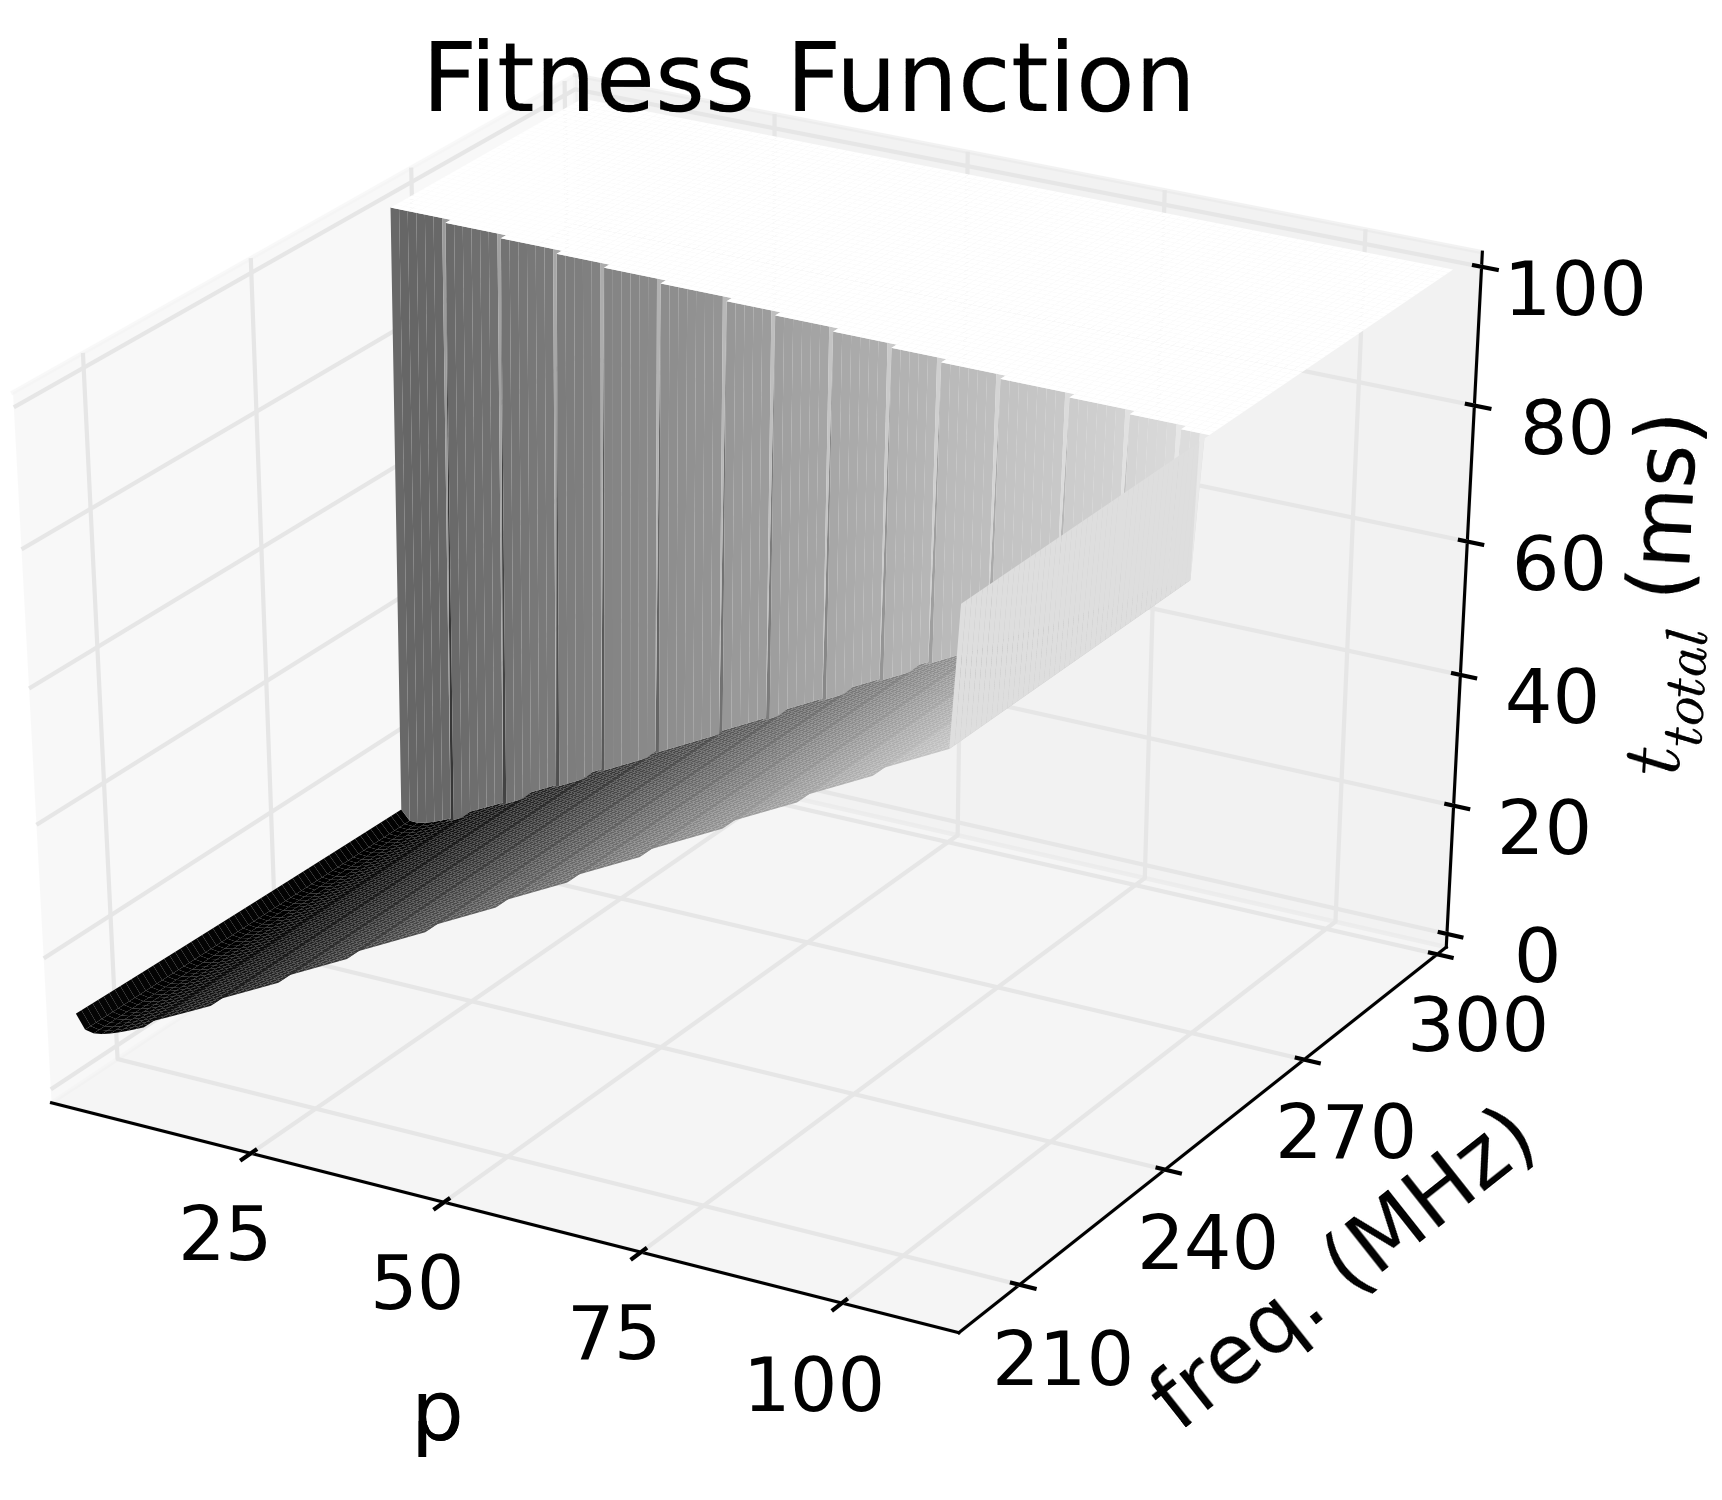
\includegraphics[width=\textwidth]{./figs/fitness1.png}
        \end{subfigure}
        \begin{subfigure}{0.31\textwidth}
                \centering
                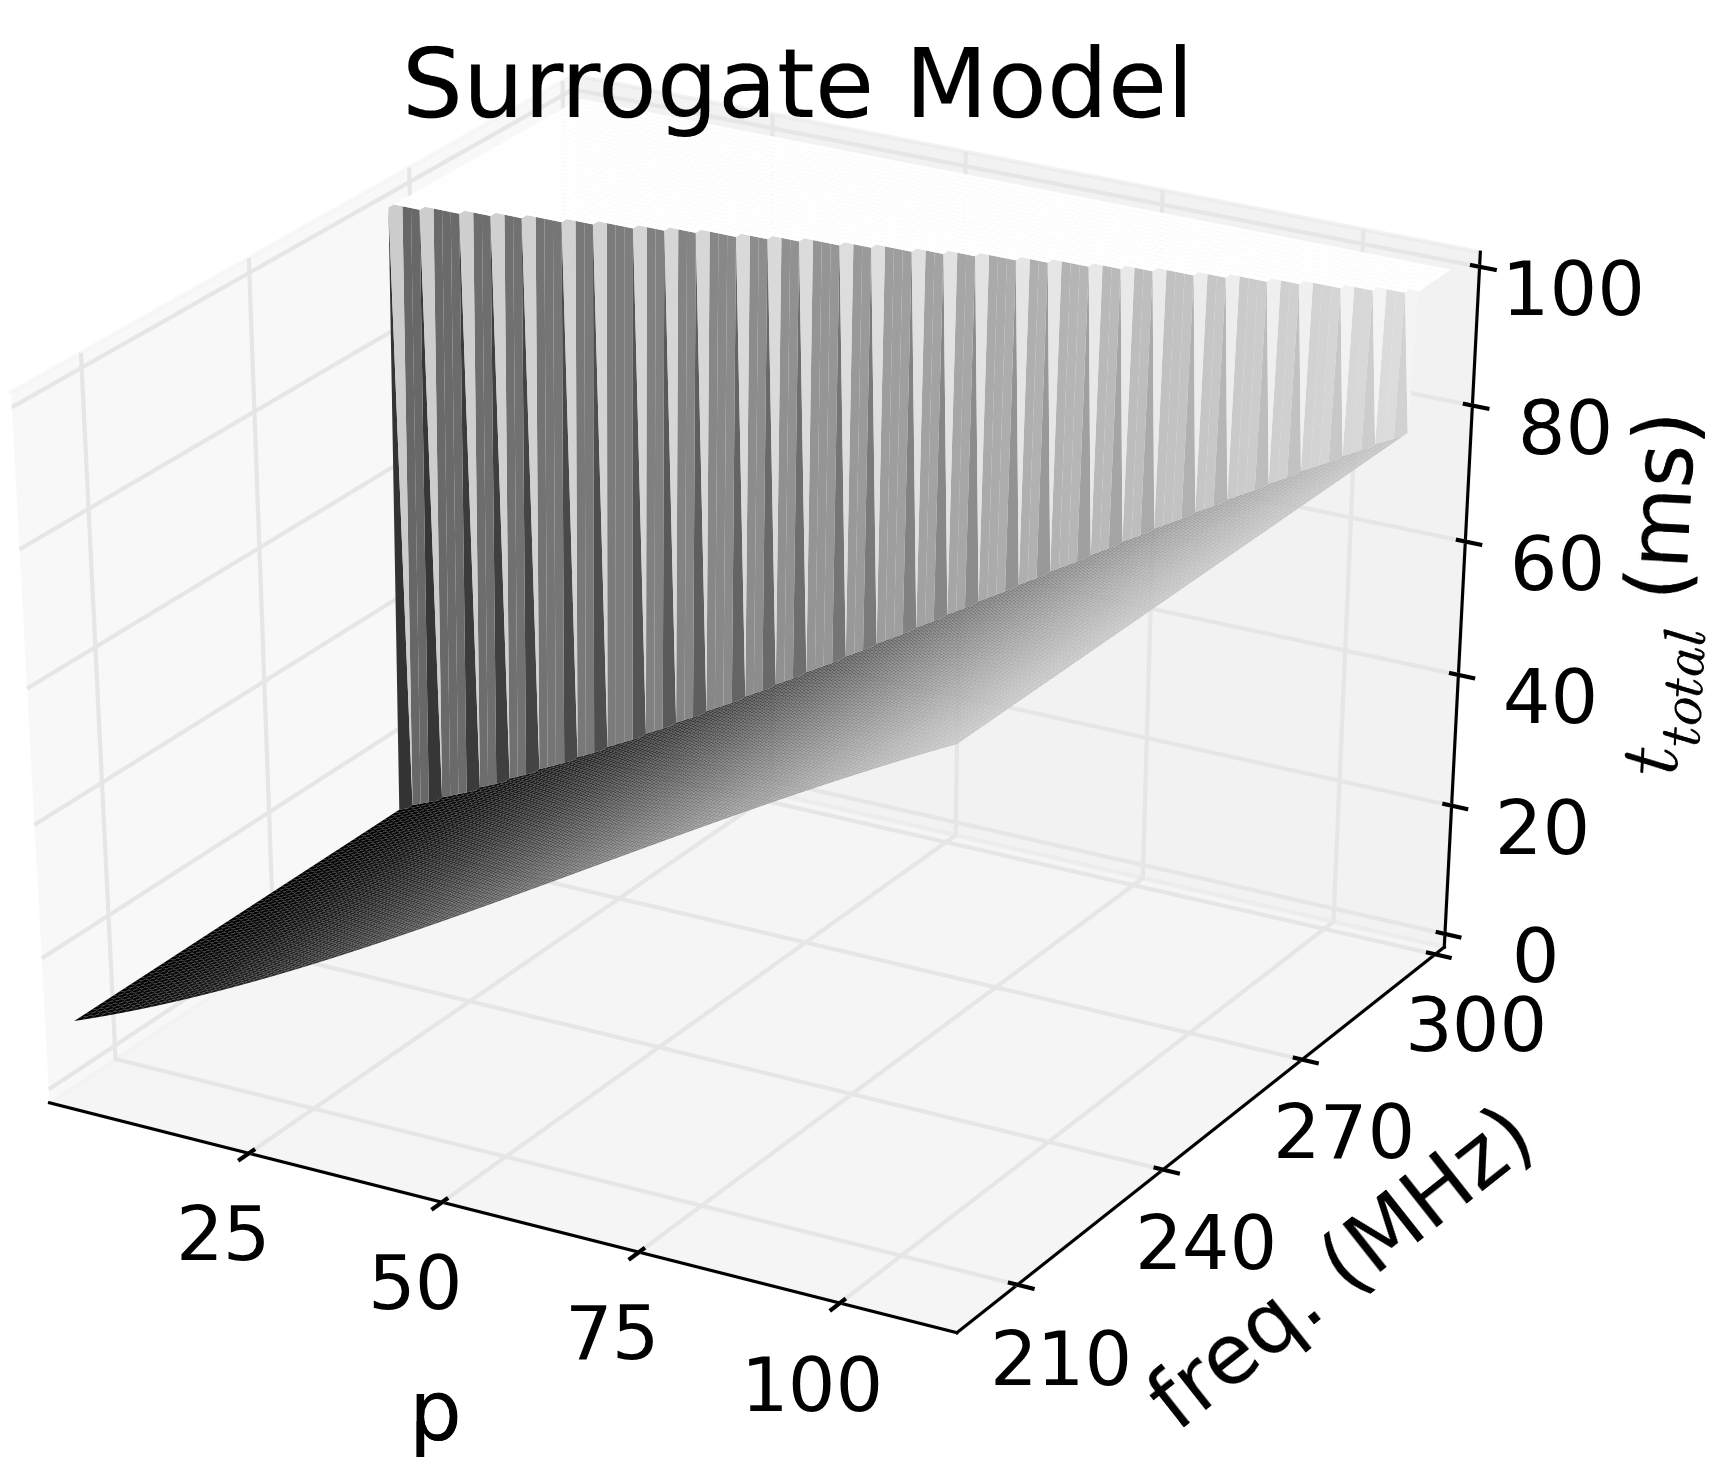
\includegraphics[width=\textwidth]{./figs/surmodel009_11.png}
        \end{subfigure}
        \begin{subfigure}{0.31\textwidth}
                \centering
                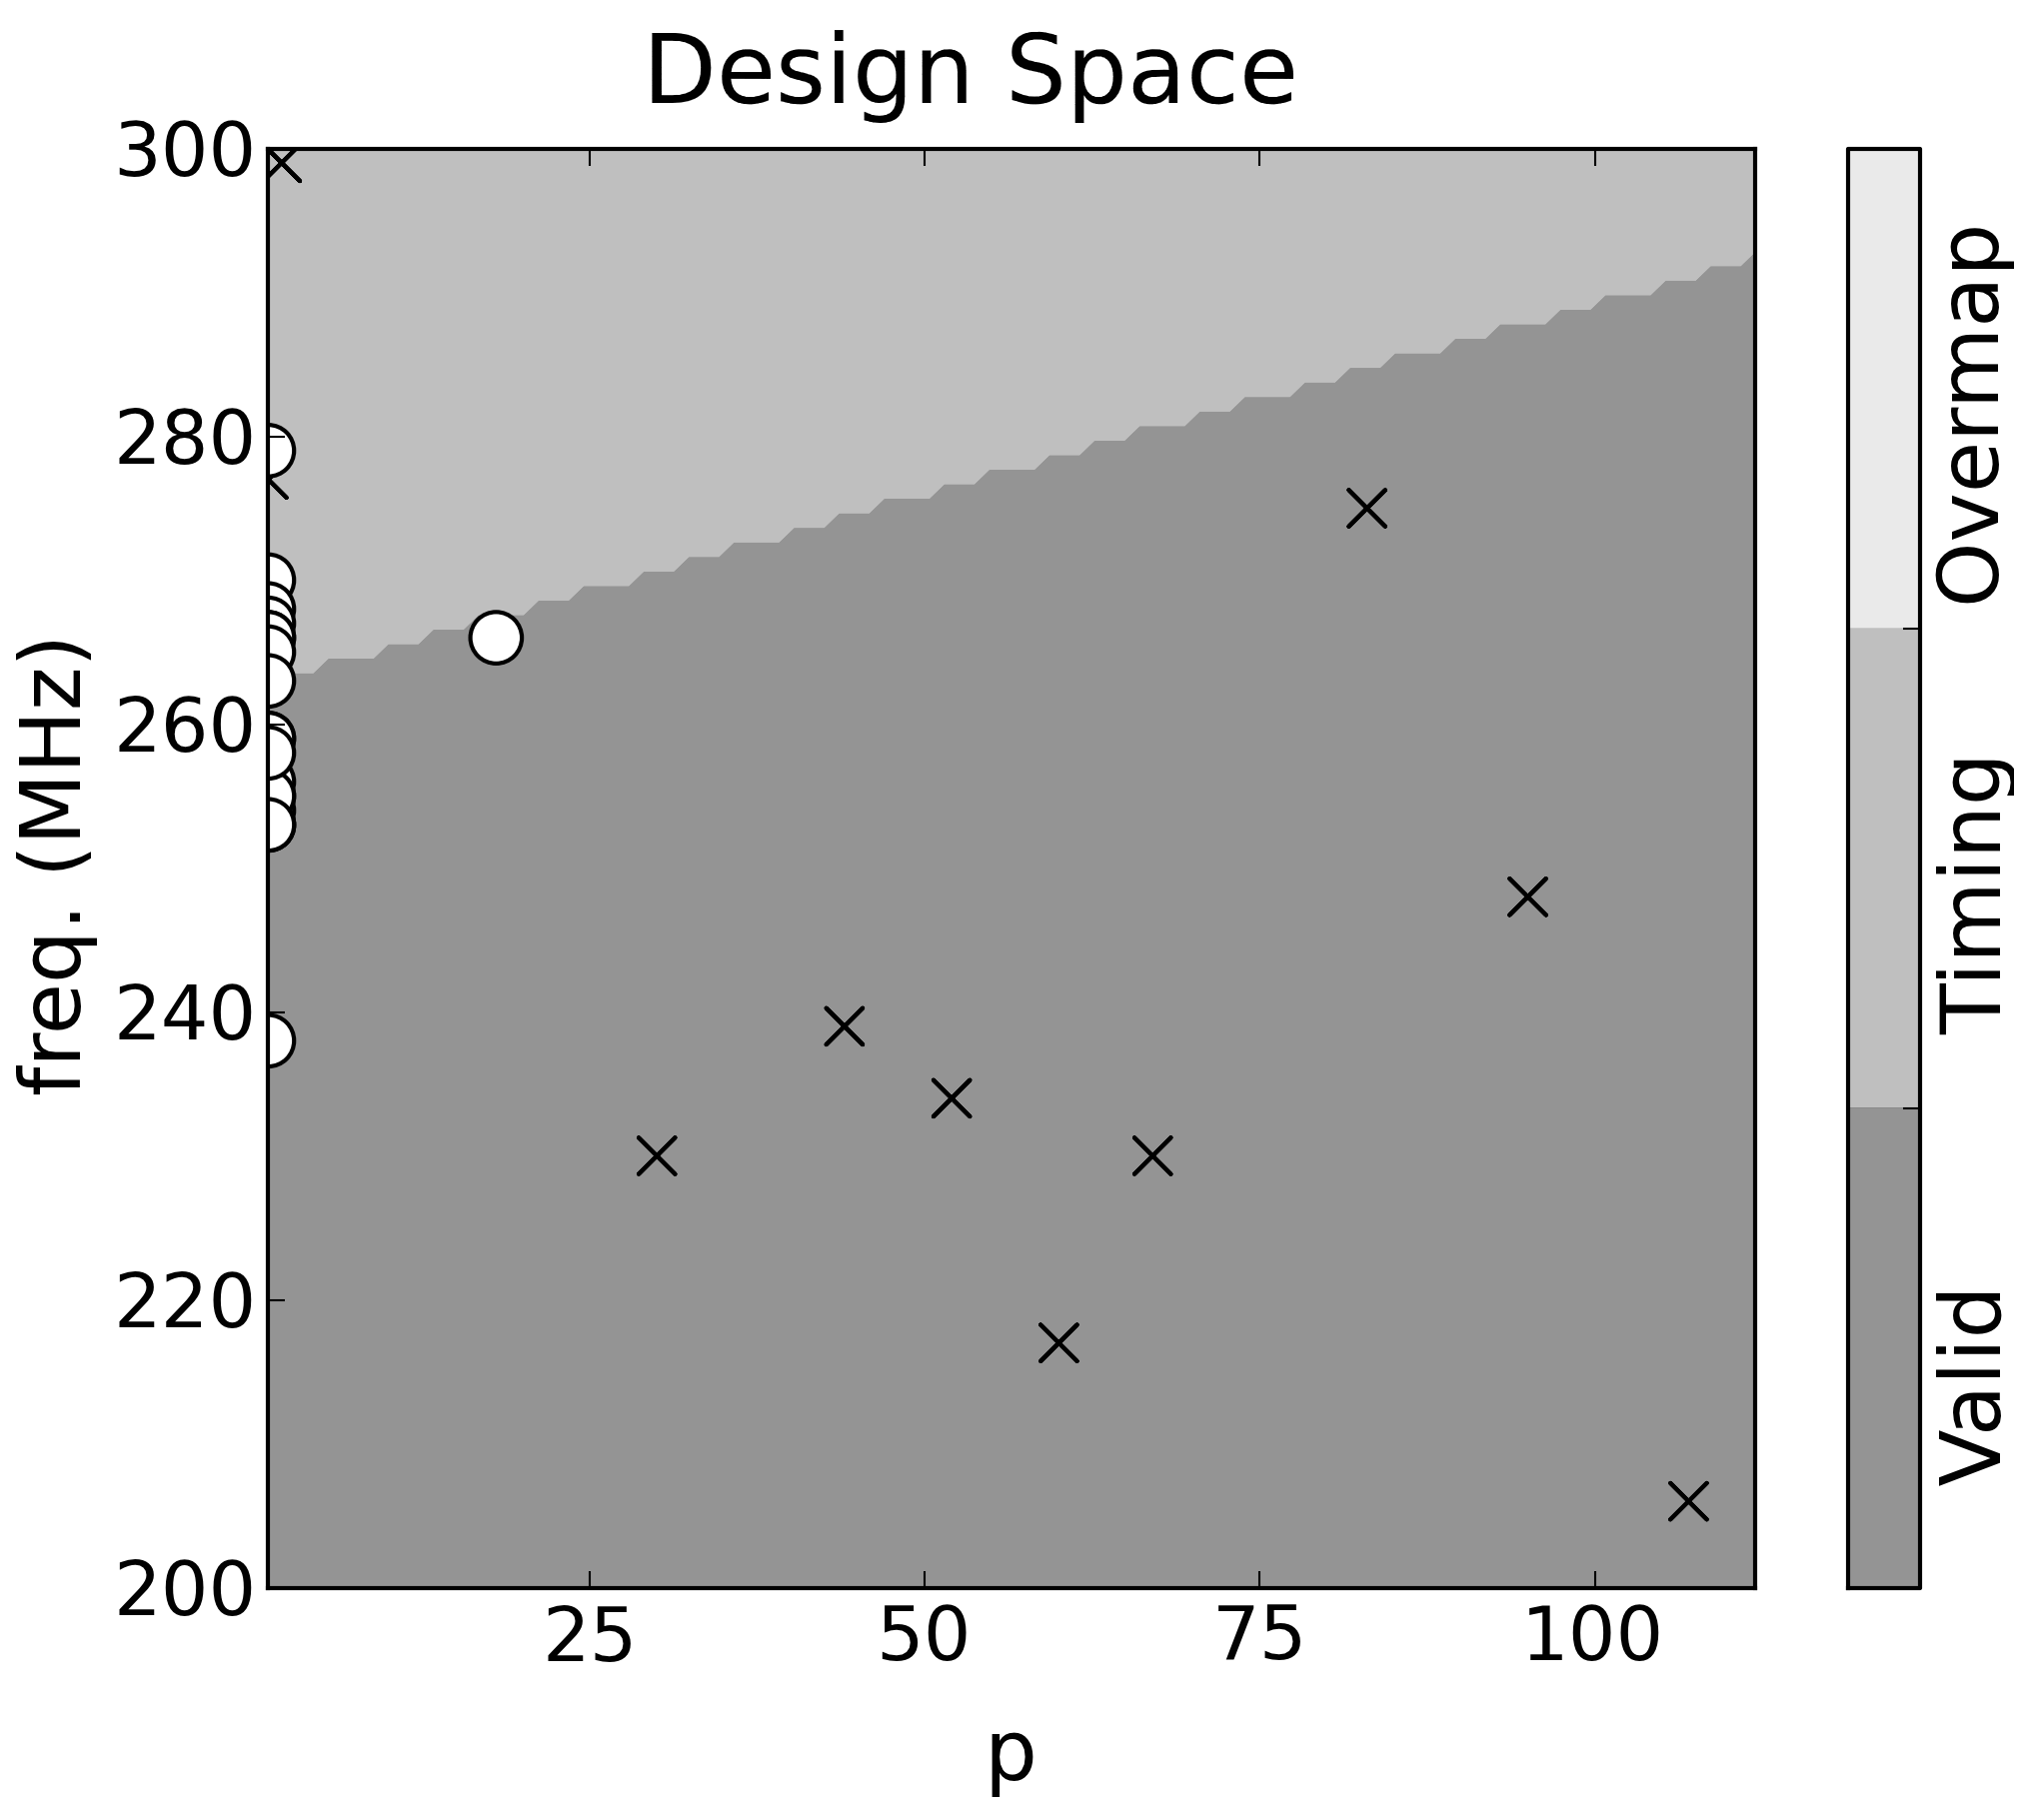
\includegraphics[width=\textwidth]{./figs/svm009_11.png}
        \end{subfigure}
        \caption{Reconfigurable radio $f$ ($\Phi_{config}$ = 5\,MB/s) and its surrogate model.}\label{fig:fitness_2}
\end{figure}

%\vspace{-3em}

\begin{figure}
        \centering
        \begin{subfigure}{0.32\textwidth}
                \centering
                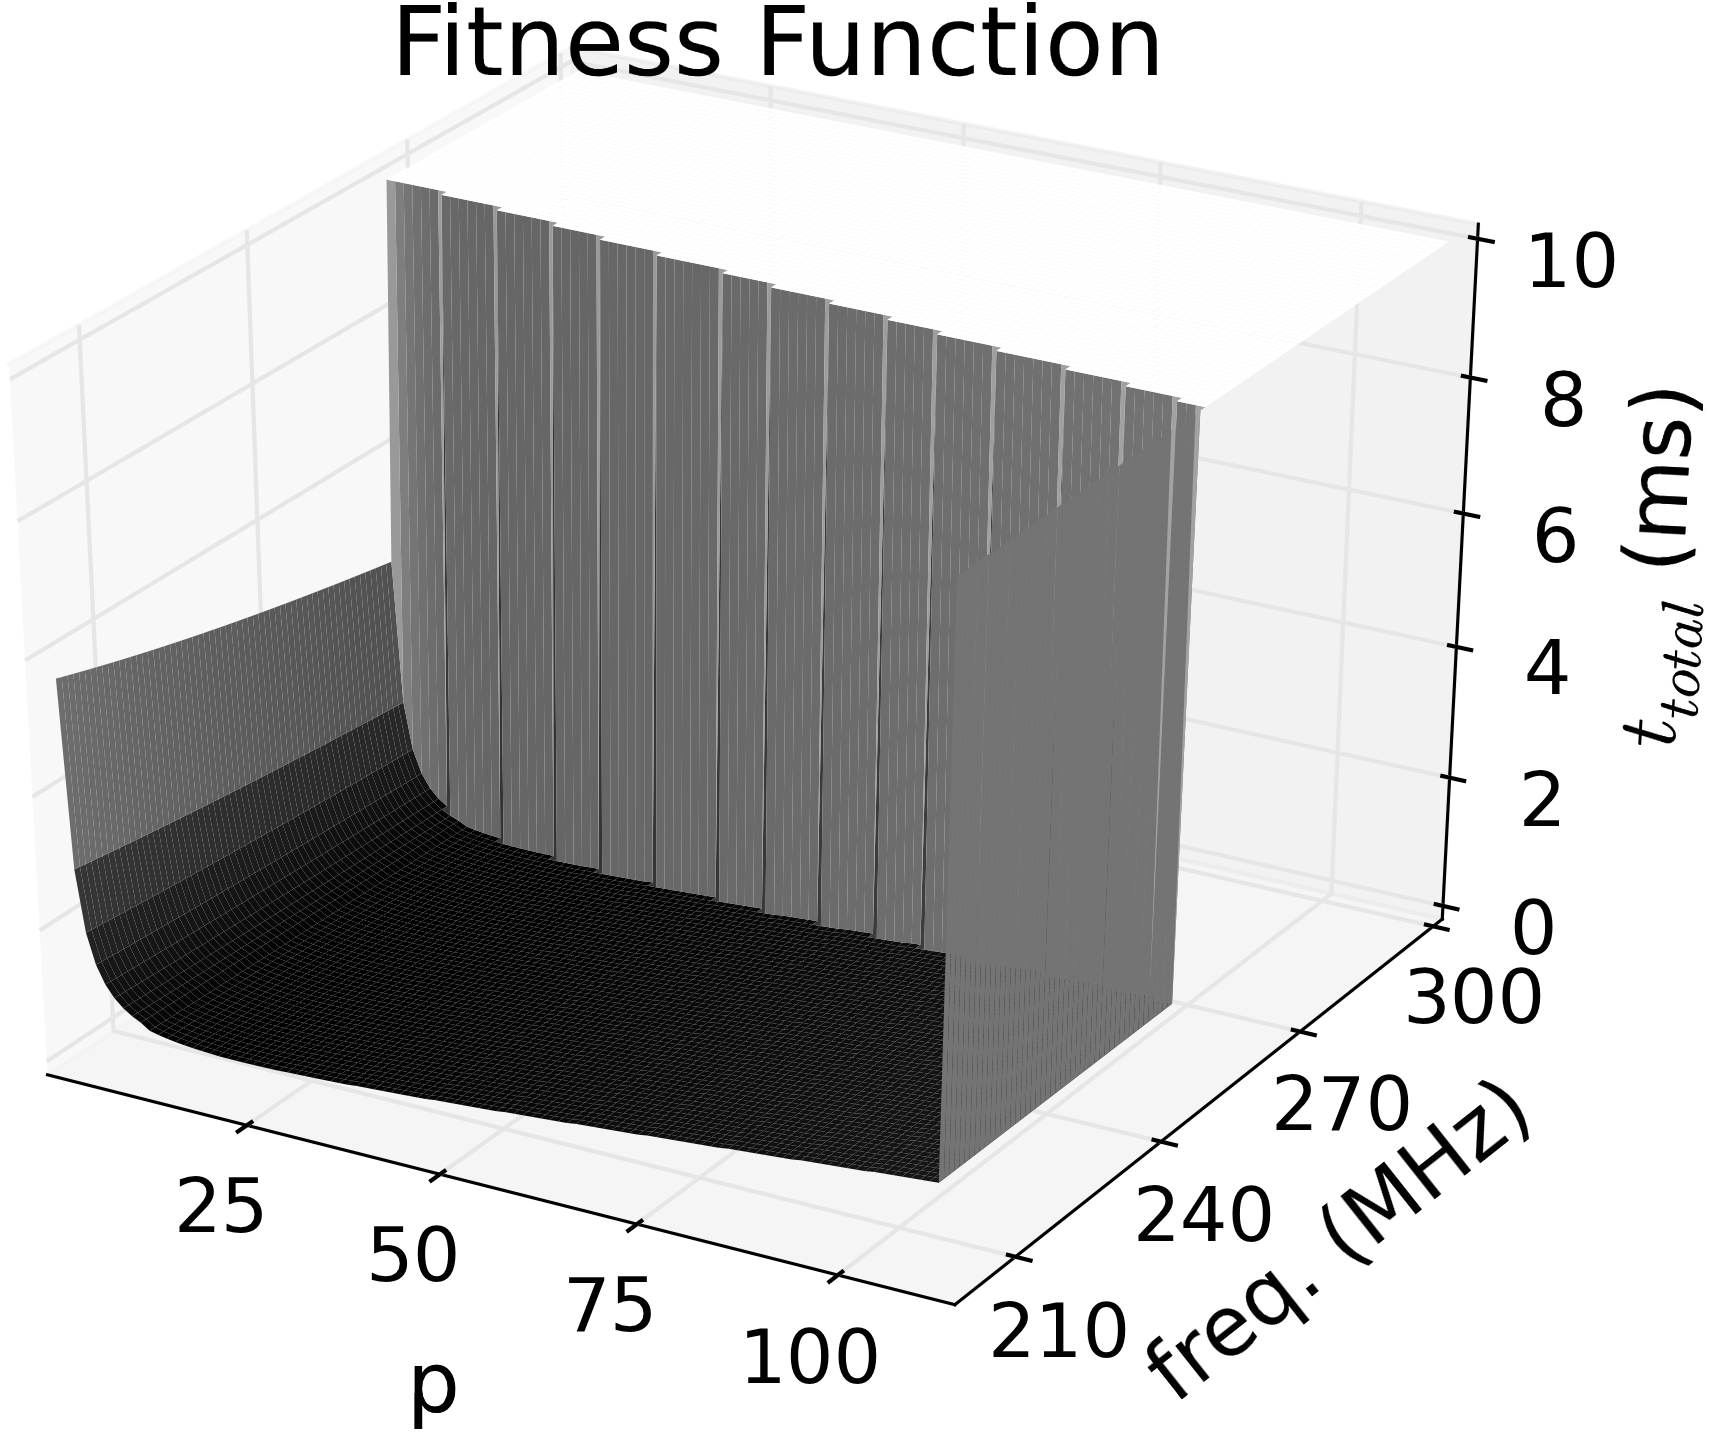
\includegraphics[width=\textwidth]{./figs/fitness_radio.png}
        \end{subfigure}
        \begin{subfigure}{0.32\textwidth}
                \centering
                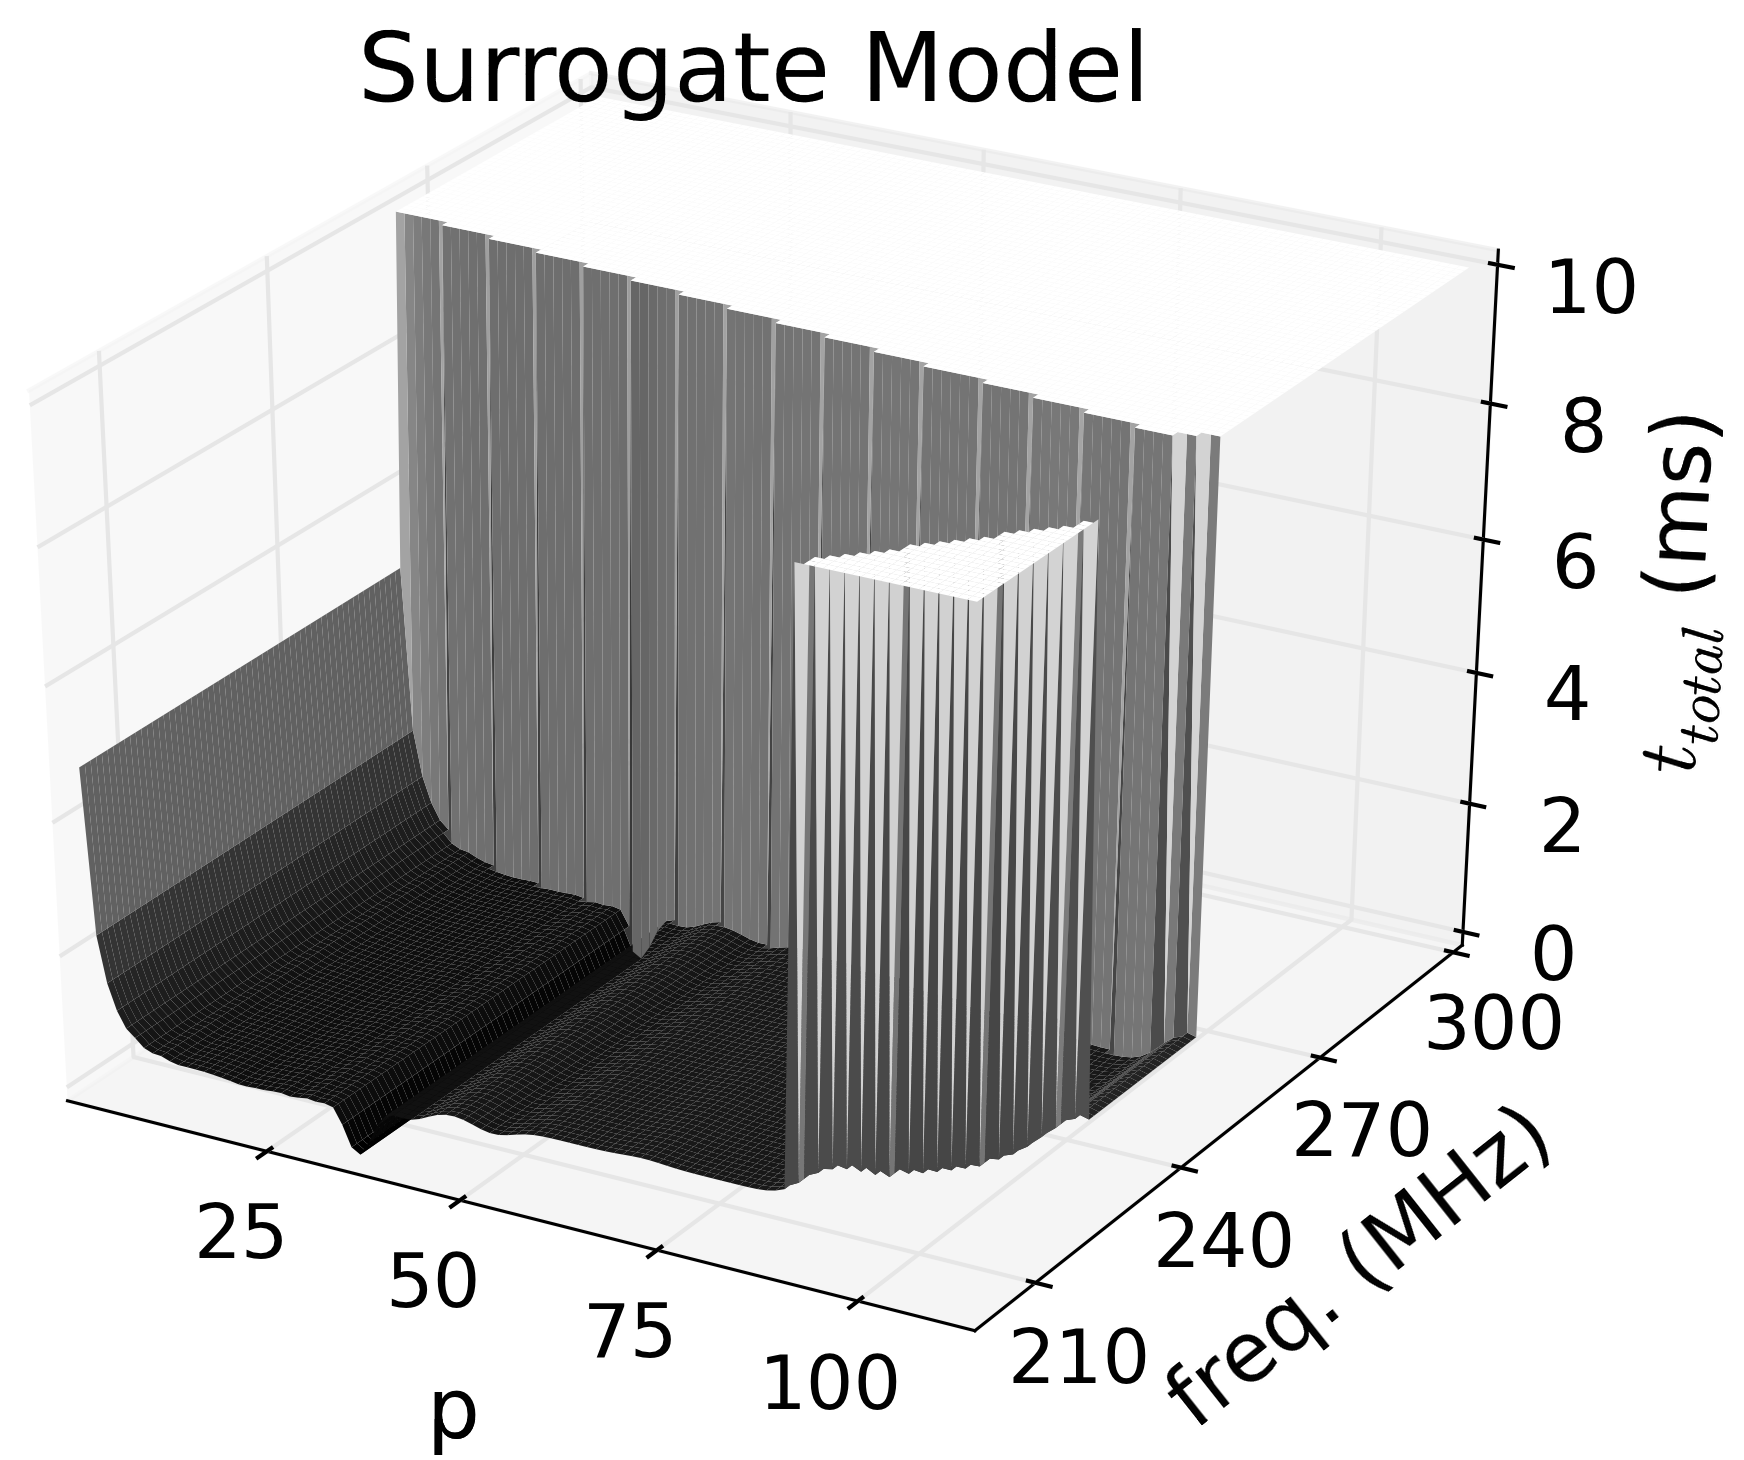
\includegraphics[width=\textwidth]{./figs/surmodel025_44.png}
        \end{subfigure}
        \begin{subfigure}{0.32\textwidth}
                \centering
                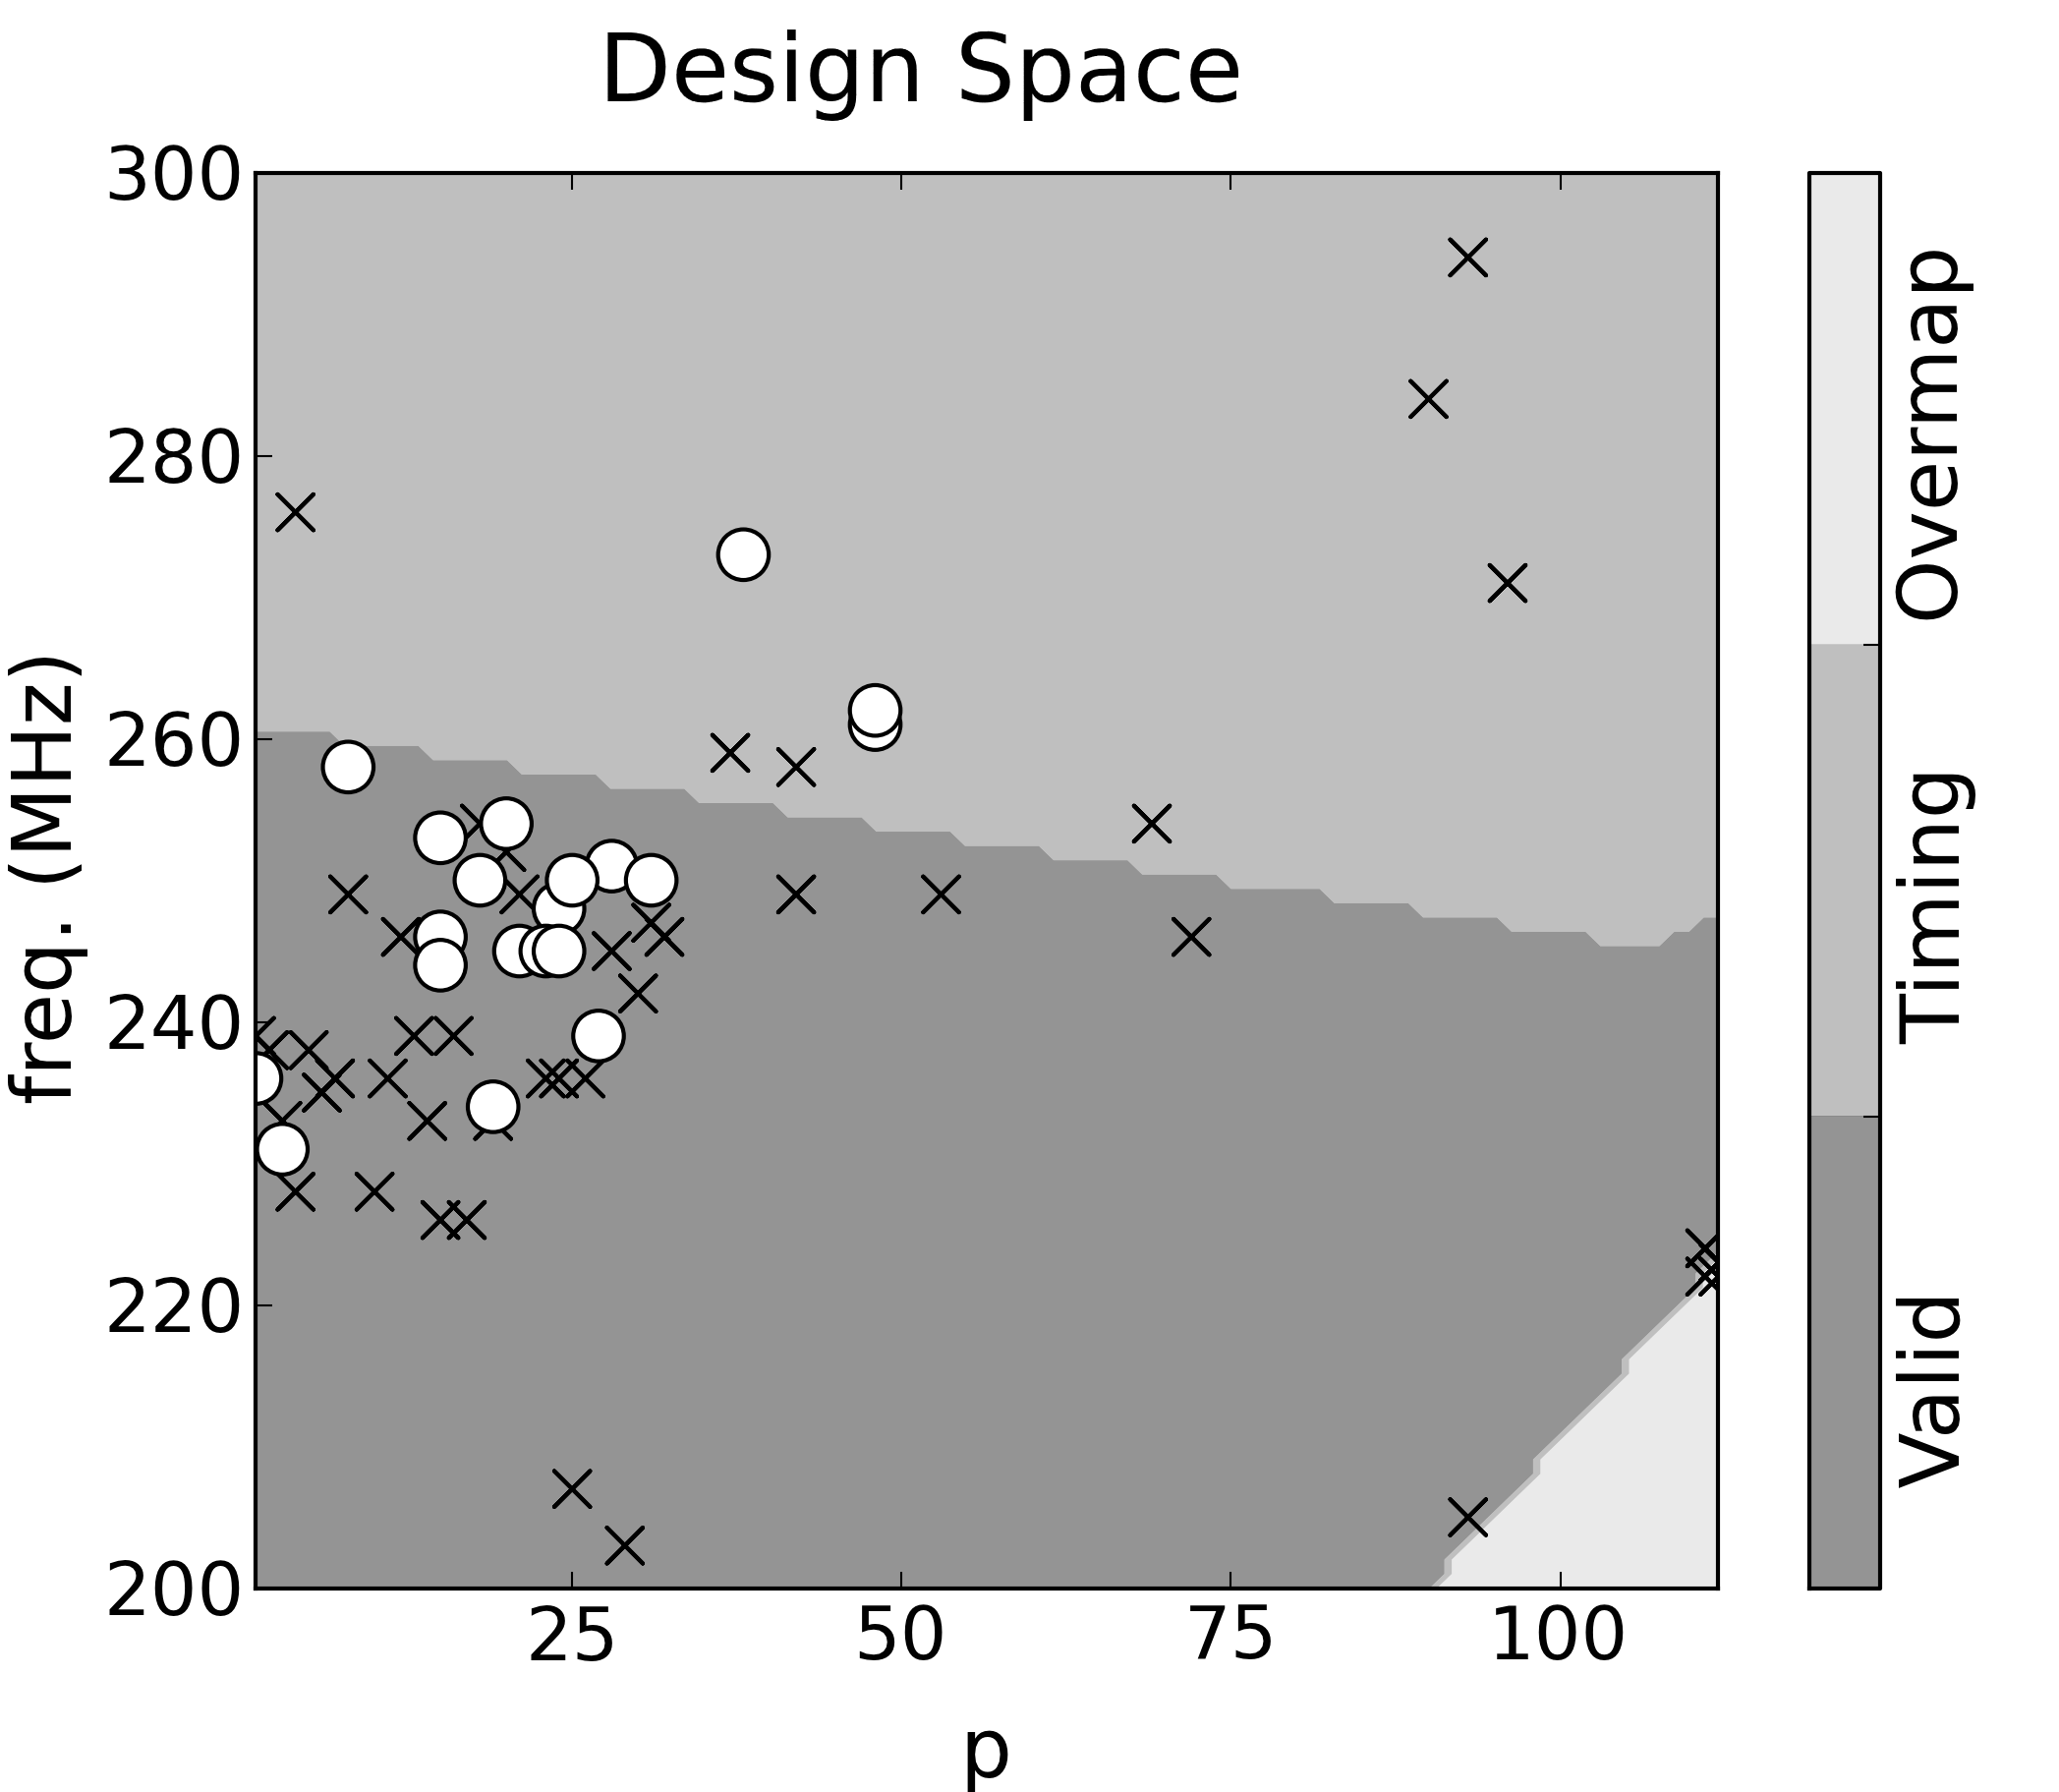
\includegraphics[width=\textwidth]{./figs/svm025_44.png}
        \end{subfigure}
        \caption{Reconfigurable radio $f$ ($\Phi_{config}$ = 300\,MB/s) and its surrogate model.}\label{fig:fitness_1}
\end{figure}

Our parameters are $p$, $\Phi_{config}$ and core frequency $freq$. We define the design space as $\mathcal{X}$ = $\{1-112\} \times \{5,300\} \times \{freq_{min}-300\}$.  We change $\mathcal{X}$ by varying the minimum frequency $freq_{min}$. Although the problem is three-dimensional, due to low discretization level of $\Phi_{config}$ we treat it as two separate two-dimensional optimizations. For the $\mathcal{I}$  region constituting timing and \ac{fpga} resource over-mapping regions, we mark the execution time as undesirable. \ac{alo} terminates when $\mathbf{x}$ is evaluated within 2\,MHz range of globally optimal solution. 


%To measure \ac{alo} convergence the optimizer terminates if the current best particle is within the 2\,MHz range of the optimal solution. Maximizing bitstream frequency is highly indeterministic   

%
%\begin{align} 
%\label{eq:radio0}
%t_{total}(p,freq)= (steps \times t_{p,e}) / p + t_{r,e} \times p \enspace .
%\end{align}


% \begin{table}
%  \caption {Parameters of Reconfigurable Radio.}  
%  \label{tab:kerpar}
%    \begin{center}
%\begin{tabular}{p{3.5cm} p{3.5cm}}
%\hline Parameter & Value Range \\ 
%\hline $p$ & 1,112 \\ 
% $frequency$ & 150\,MHz - 300\,MHz \\ 
% $\Phi_{config}$ & 5MB/s or 300MB/s \\
%\hline 
%\end{tabular} 
%\end{center}
%\end{table}
  
%    \begin{figure}
%     \centering
%\includegraphics[width=0.45\textwidth]{graphics/posteval.png}
%        \caption{Visualization of \ac{alo} state after X Fitness Function evaluations. ($frequency$ 200-300\,MHz,$\Phi_{config}$ = 300\,MB/s)}     
%           \label{fig:ouridea}
%  \end{figure}  

%Our algorithm manages to find the optimal setting with minimal user input, the benchmark application and associated goals. Our model is generi

 % $area < max_{area}$ if $p<113$, i.e. the bitstream generation fails for more then 112 steps.

%\multicolumn{4}{l}{$max_{stdv}$ = 0.05, $\Phi_{config}$ = 5\,MB/s} \\ 
%\hline 0.01 & 64 & 80 & 61 \\
%       0.05 & 39 & 39 & 44 \\ 
%       0.10 & 34 & 42 & 31 \\ 
%\hline  
%\multicolumn{4}{l}{$max_{stdv}$ = 0.01, $\Phi_{config}$ = 300\,MB/s}\\
%\hline 0.01 & 33 & 37 & 23 \\ 
%       0.05 & 44 & 35 & 41 \\ 
%       0.10 & 47 & 54 & 45 \\ 
%\hline  
%\multicolumn{4}{l}{$max_{stdv}$ = 0.05, $\Phi_{config}$ = 300\,MB/s}\\ 
%\hline 0.01 & 38 & 53 & 31 \\ 
%       0.05 & 45 & 47 & 32 \\ 
%       0.10 & 50 & 31 & 46 \\ 
%\hline 

%The $t_{total}$ function is the $y$ function according to our definition. For $\Phi_{config}$ = 300\,MB/s \ac{alo} performs substantially better then $\Phi_{config}$ = 5\,MB/s. Partial explanation is that $t_{total}$ is a sum of a linear and reciprocal function, in the $\Phi_{config}$ = 300\,MB/s case the linear component is dominant but for low $p$ and often wrongly is treated as noise. 

\begin{figure}
        \centering
        \begin{subfigure}{0.31\textwidth}
                \centering
                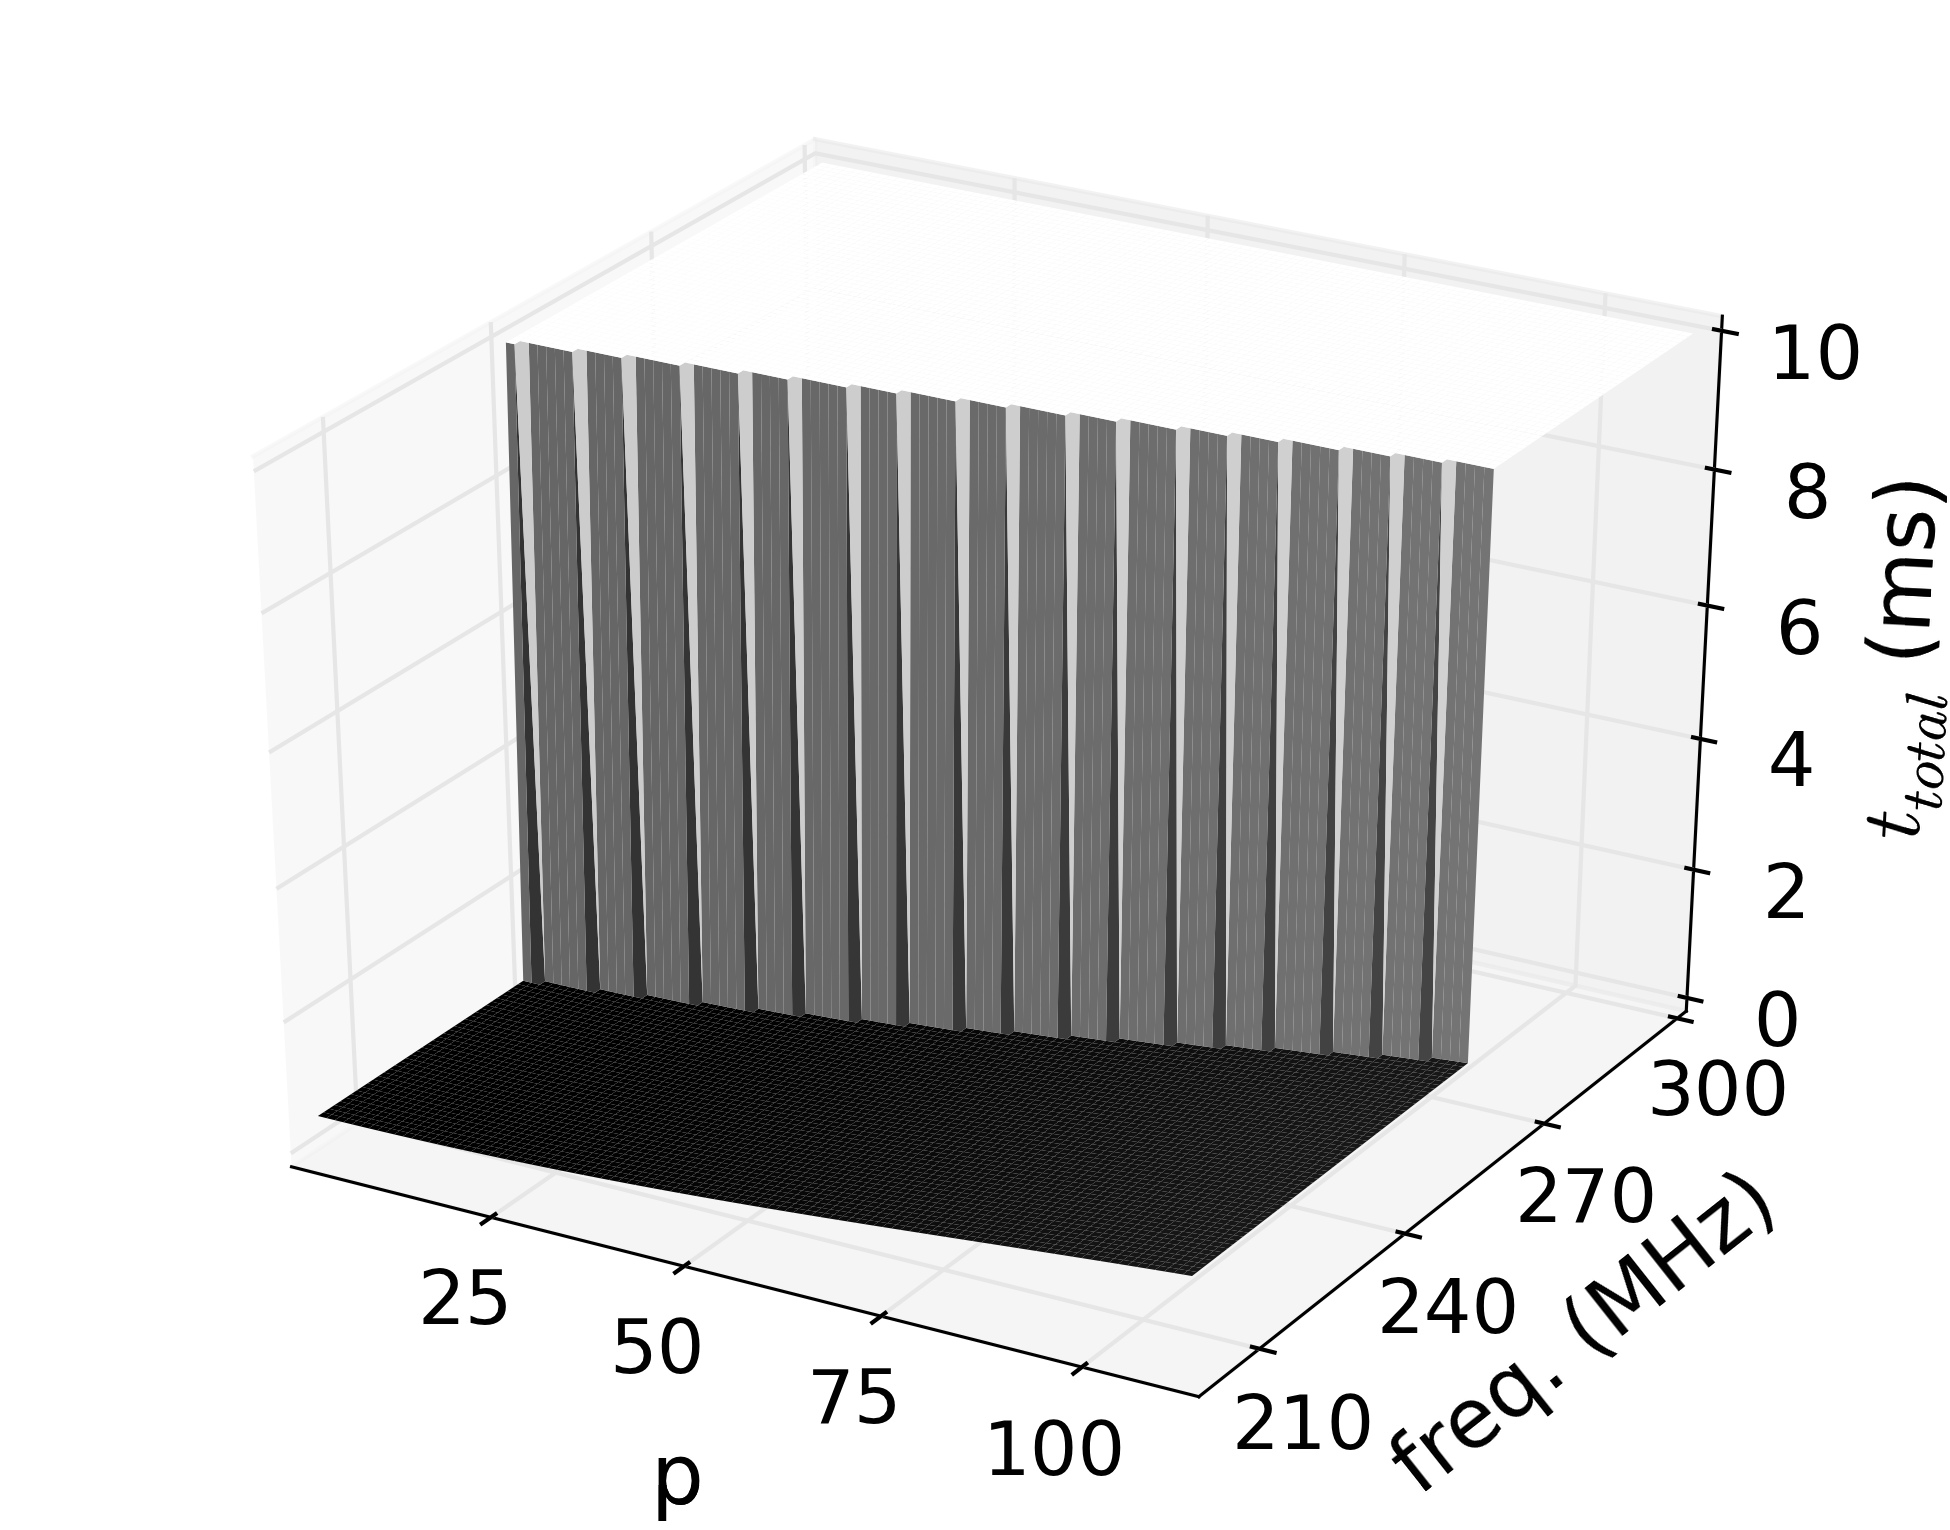
\includegraphics[width=\textwidth]{./figs/surmodel000_13.png}
        \end{subfigure}
        \begin{subfigure}{0.31\textwidth}
                \centering
                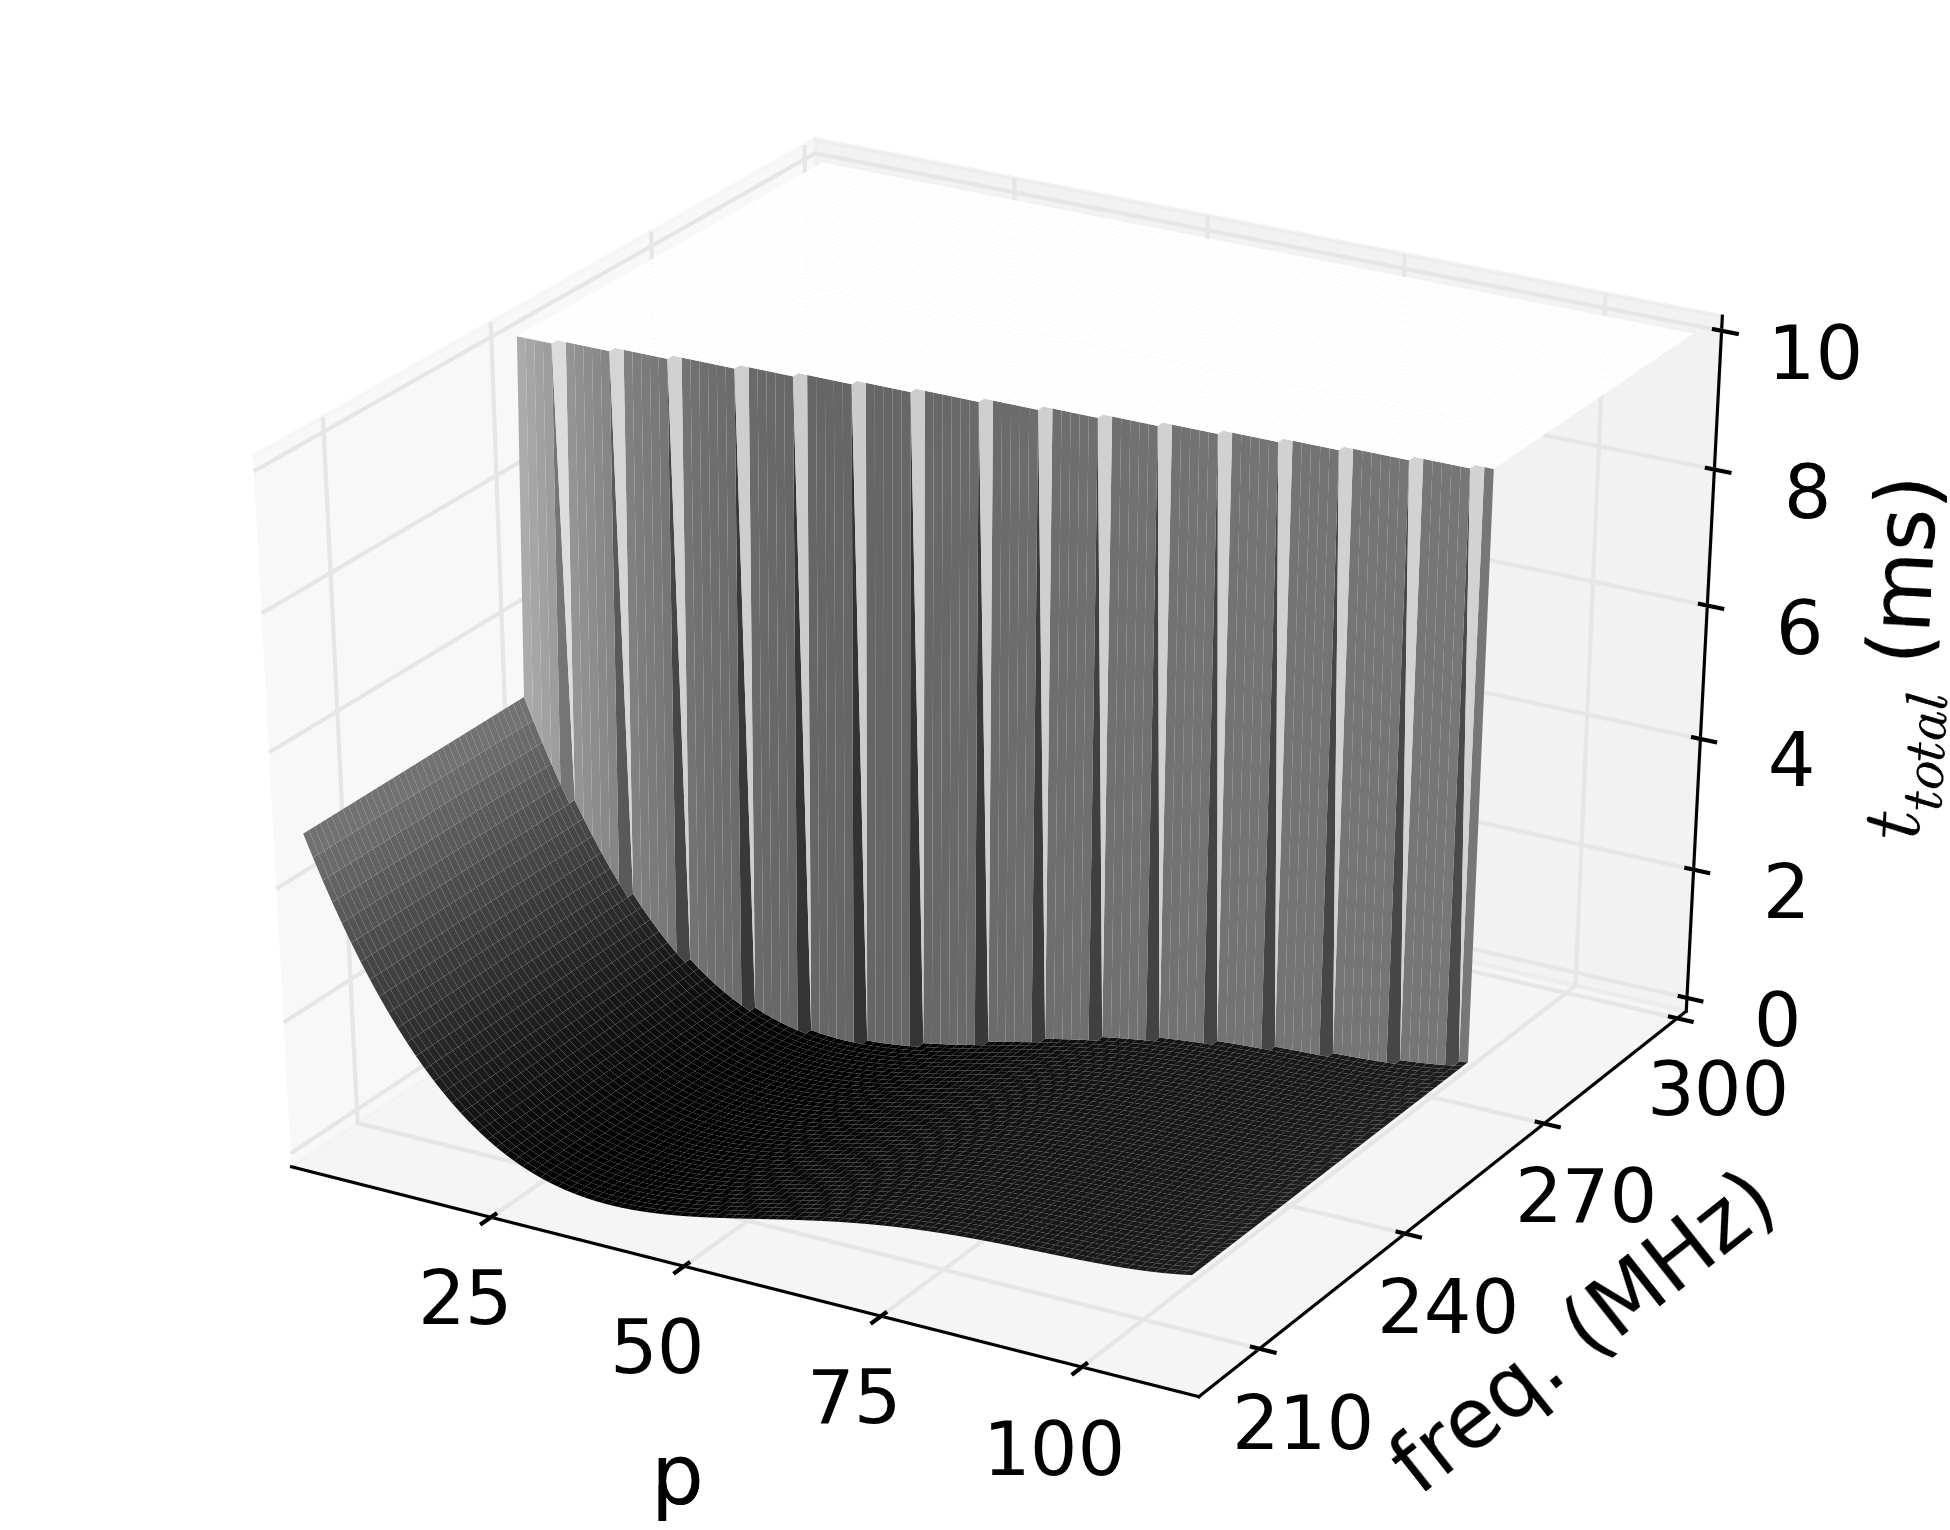
\includegraphics[width=\textwidth]{./figs/surmodel009_14.png}
        \end{subfigure}
        \begin{subfigure}{0.31\textwidth}
                \centering
                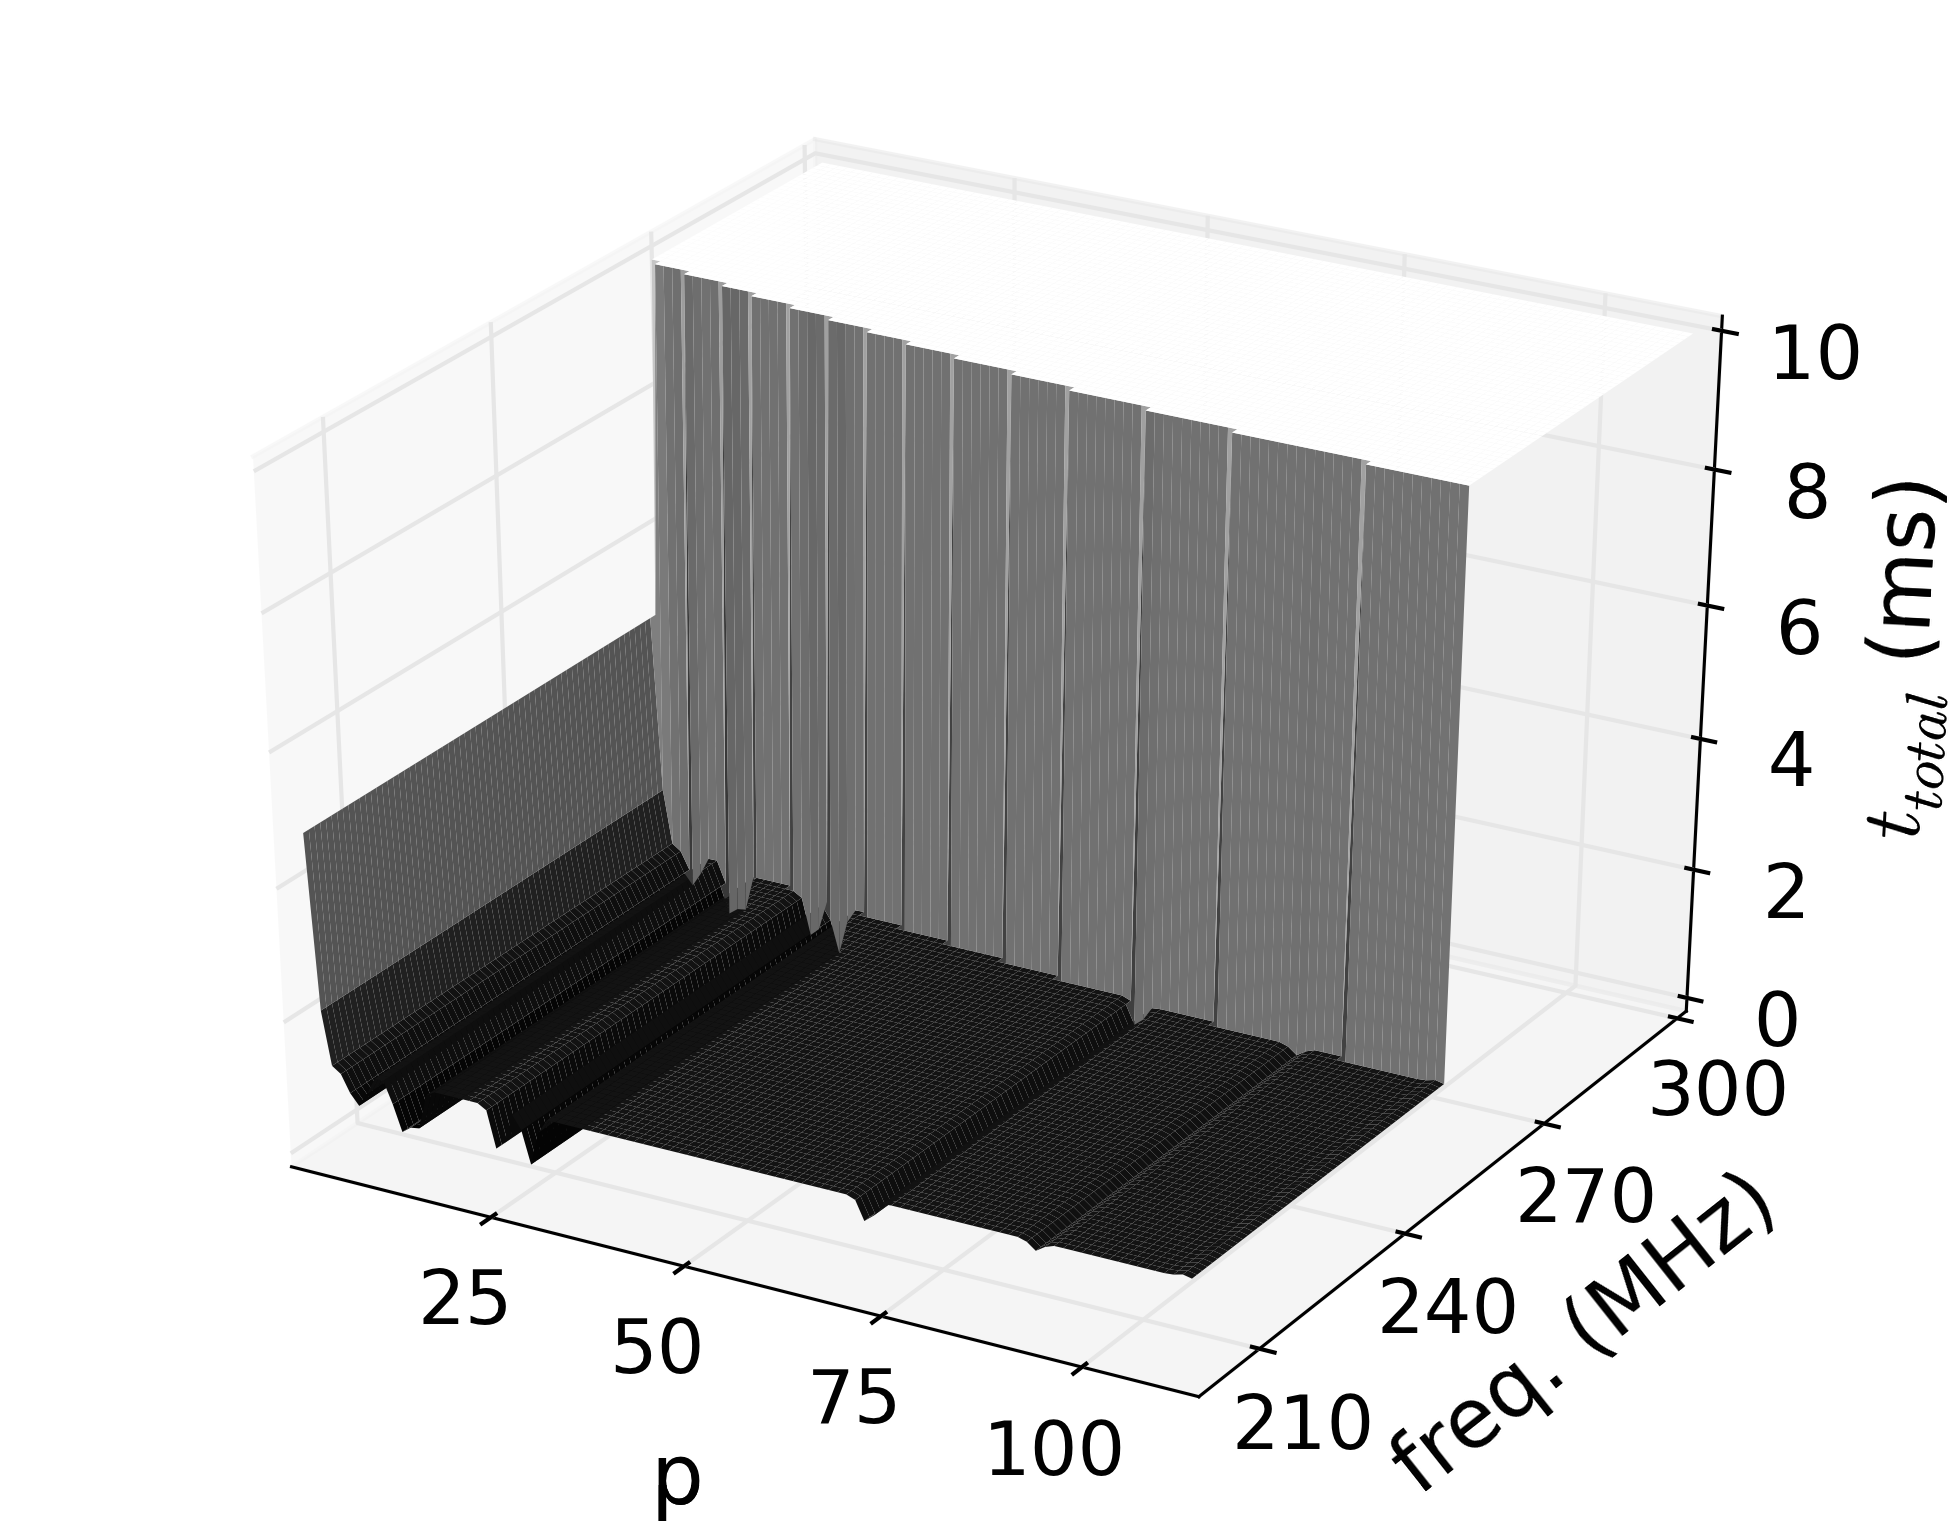
\includegraphics[width=\textwidth]{./figs/surmodel011_22.png}
        \end{subfigure}
                \begin{subfigure}{0.31\textwidth}
                \centering
                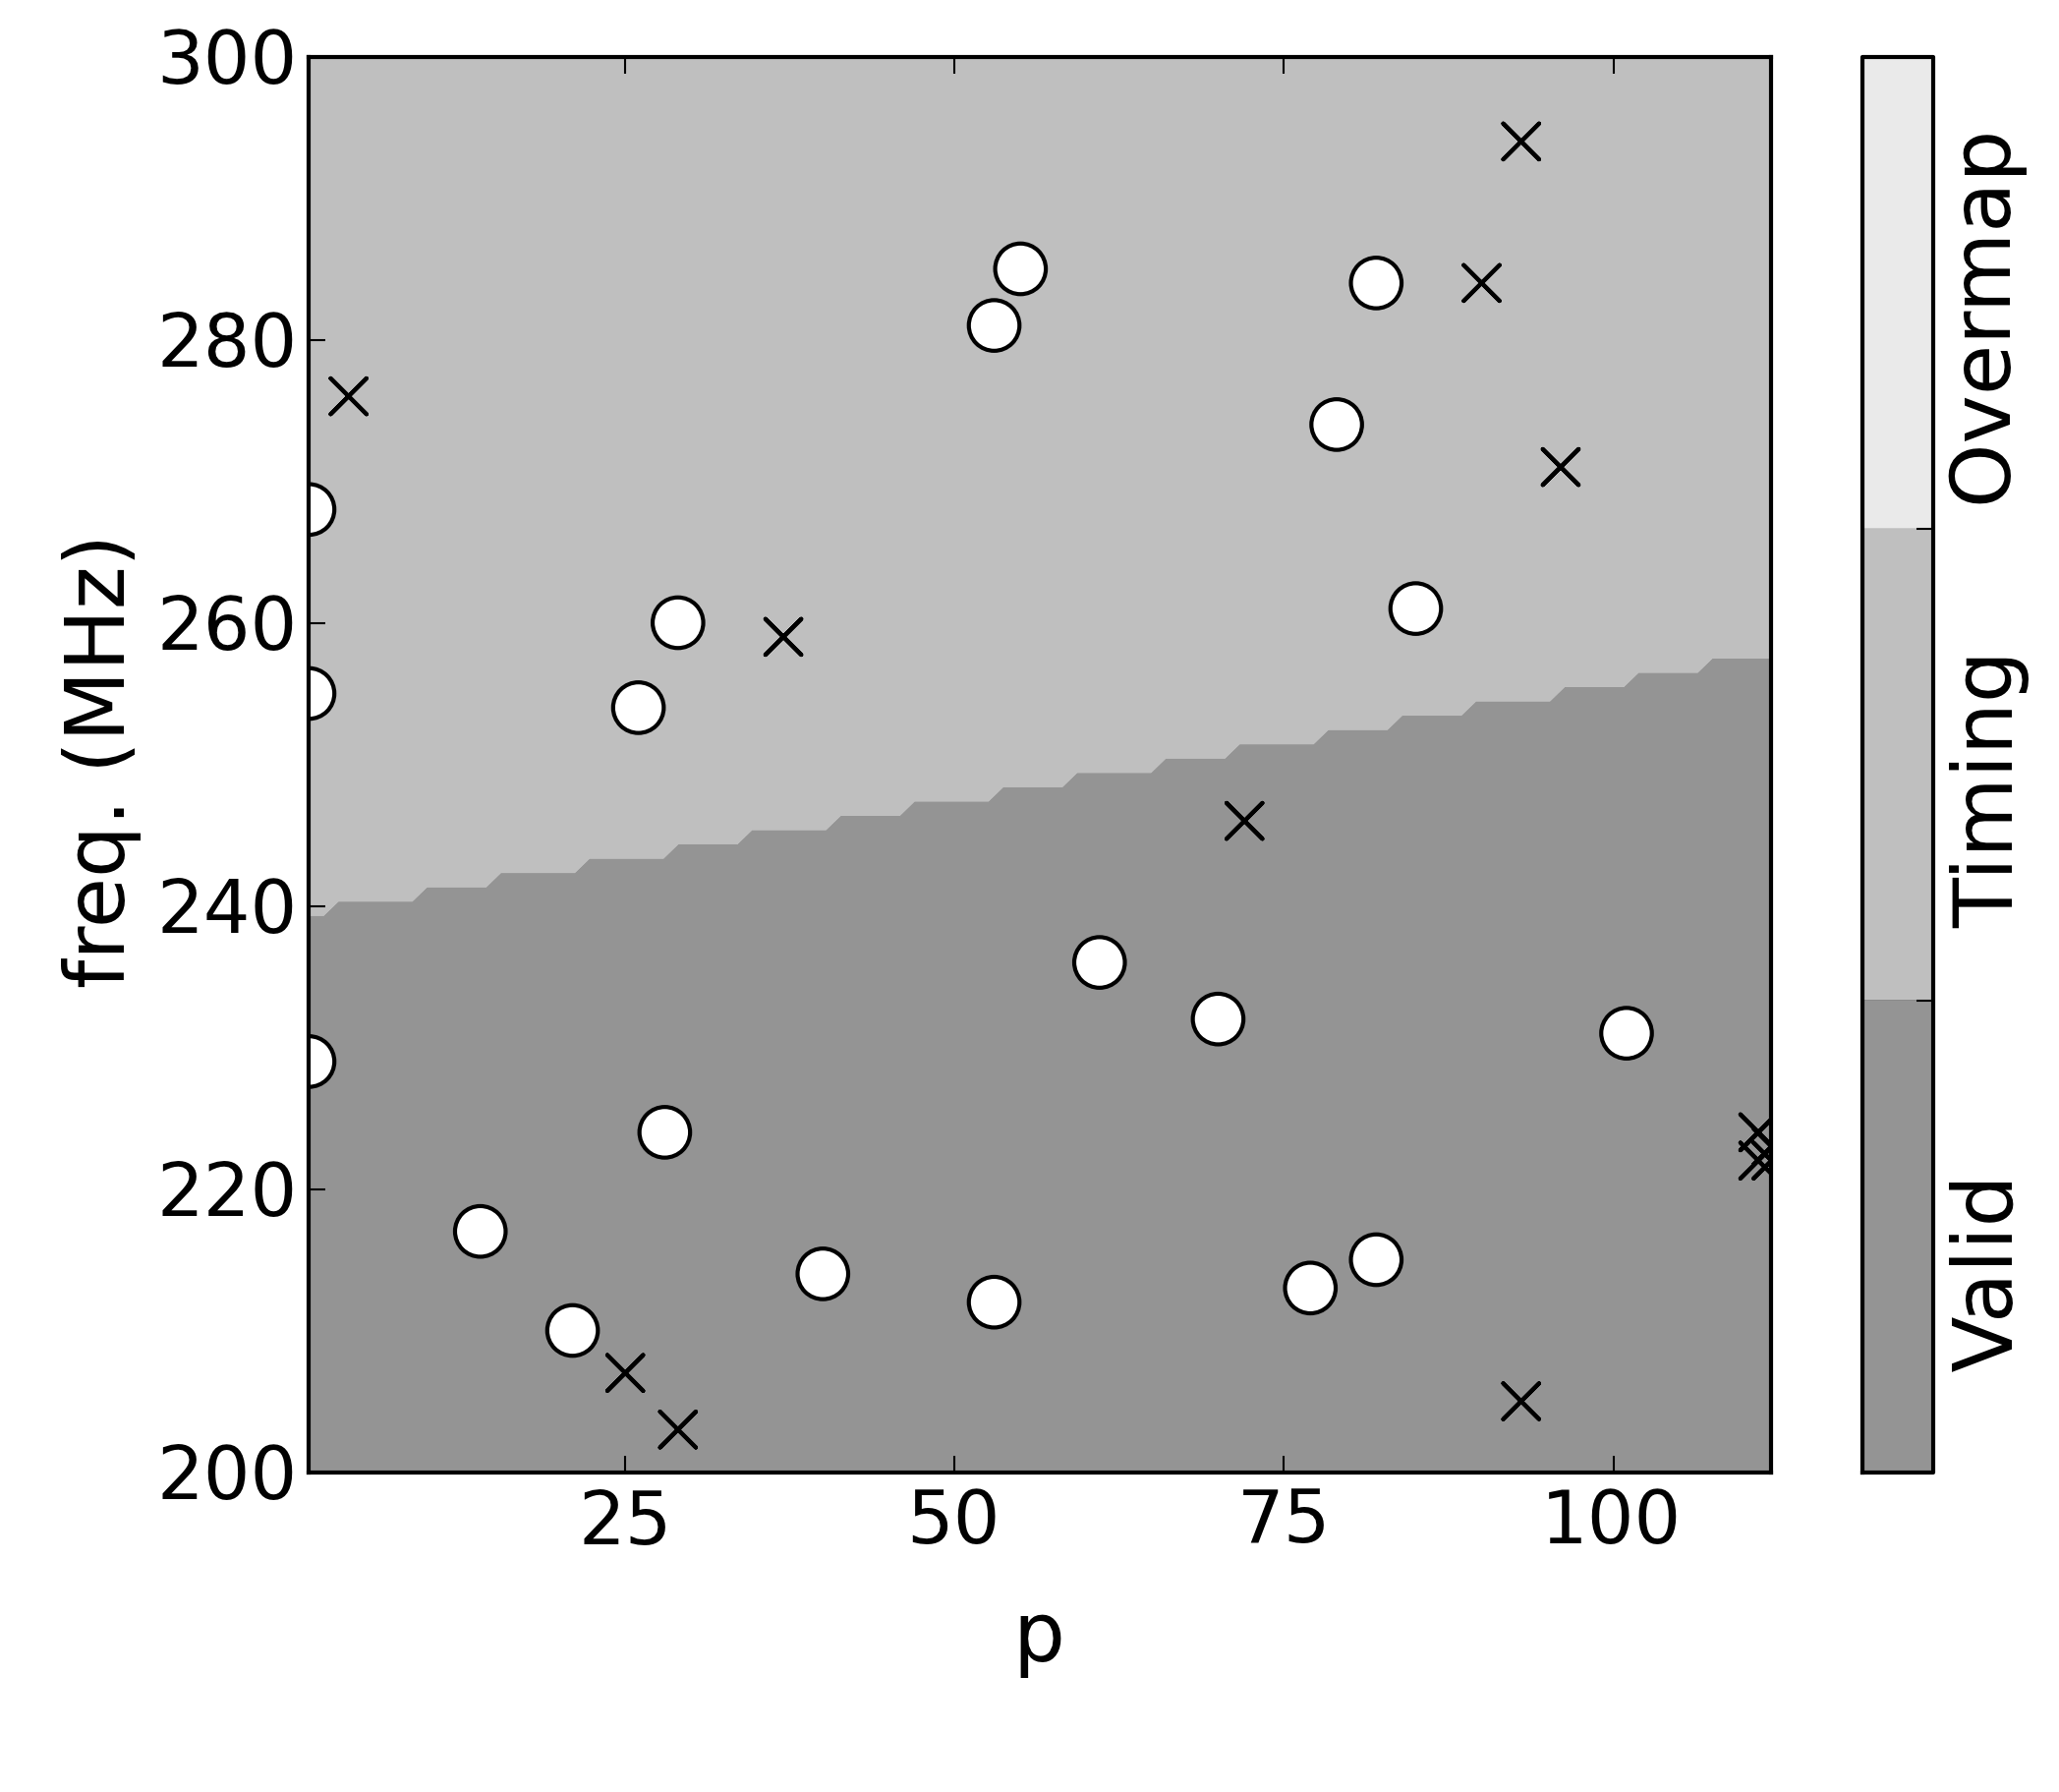
\includegraphics[width=\textwidth]{./figs/svm000_13.png}
        \end{subfigure}
        \begin{subfigure}{0.31\textwidth}
                \centering
                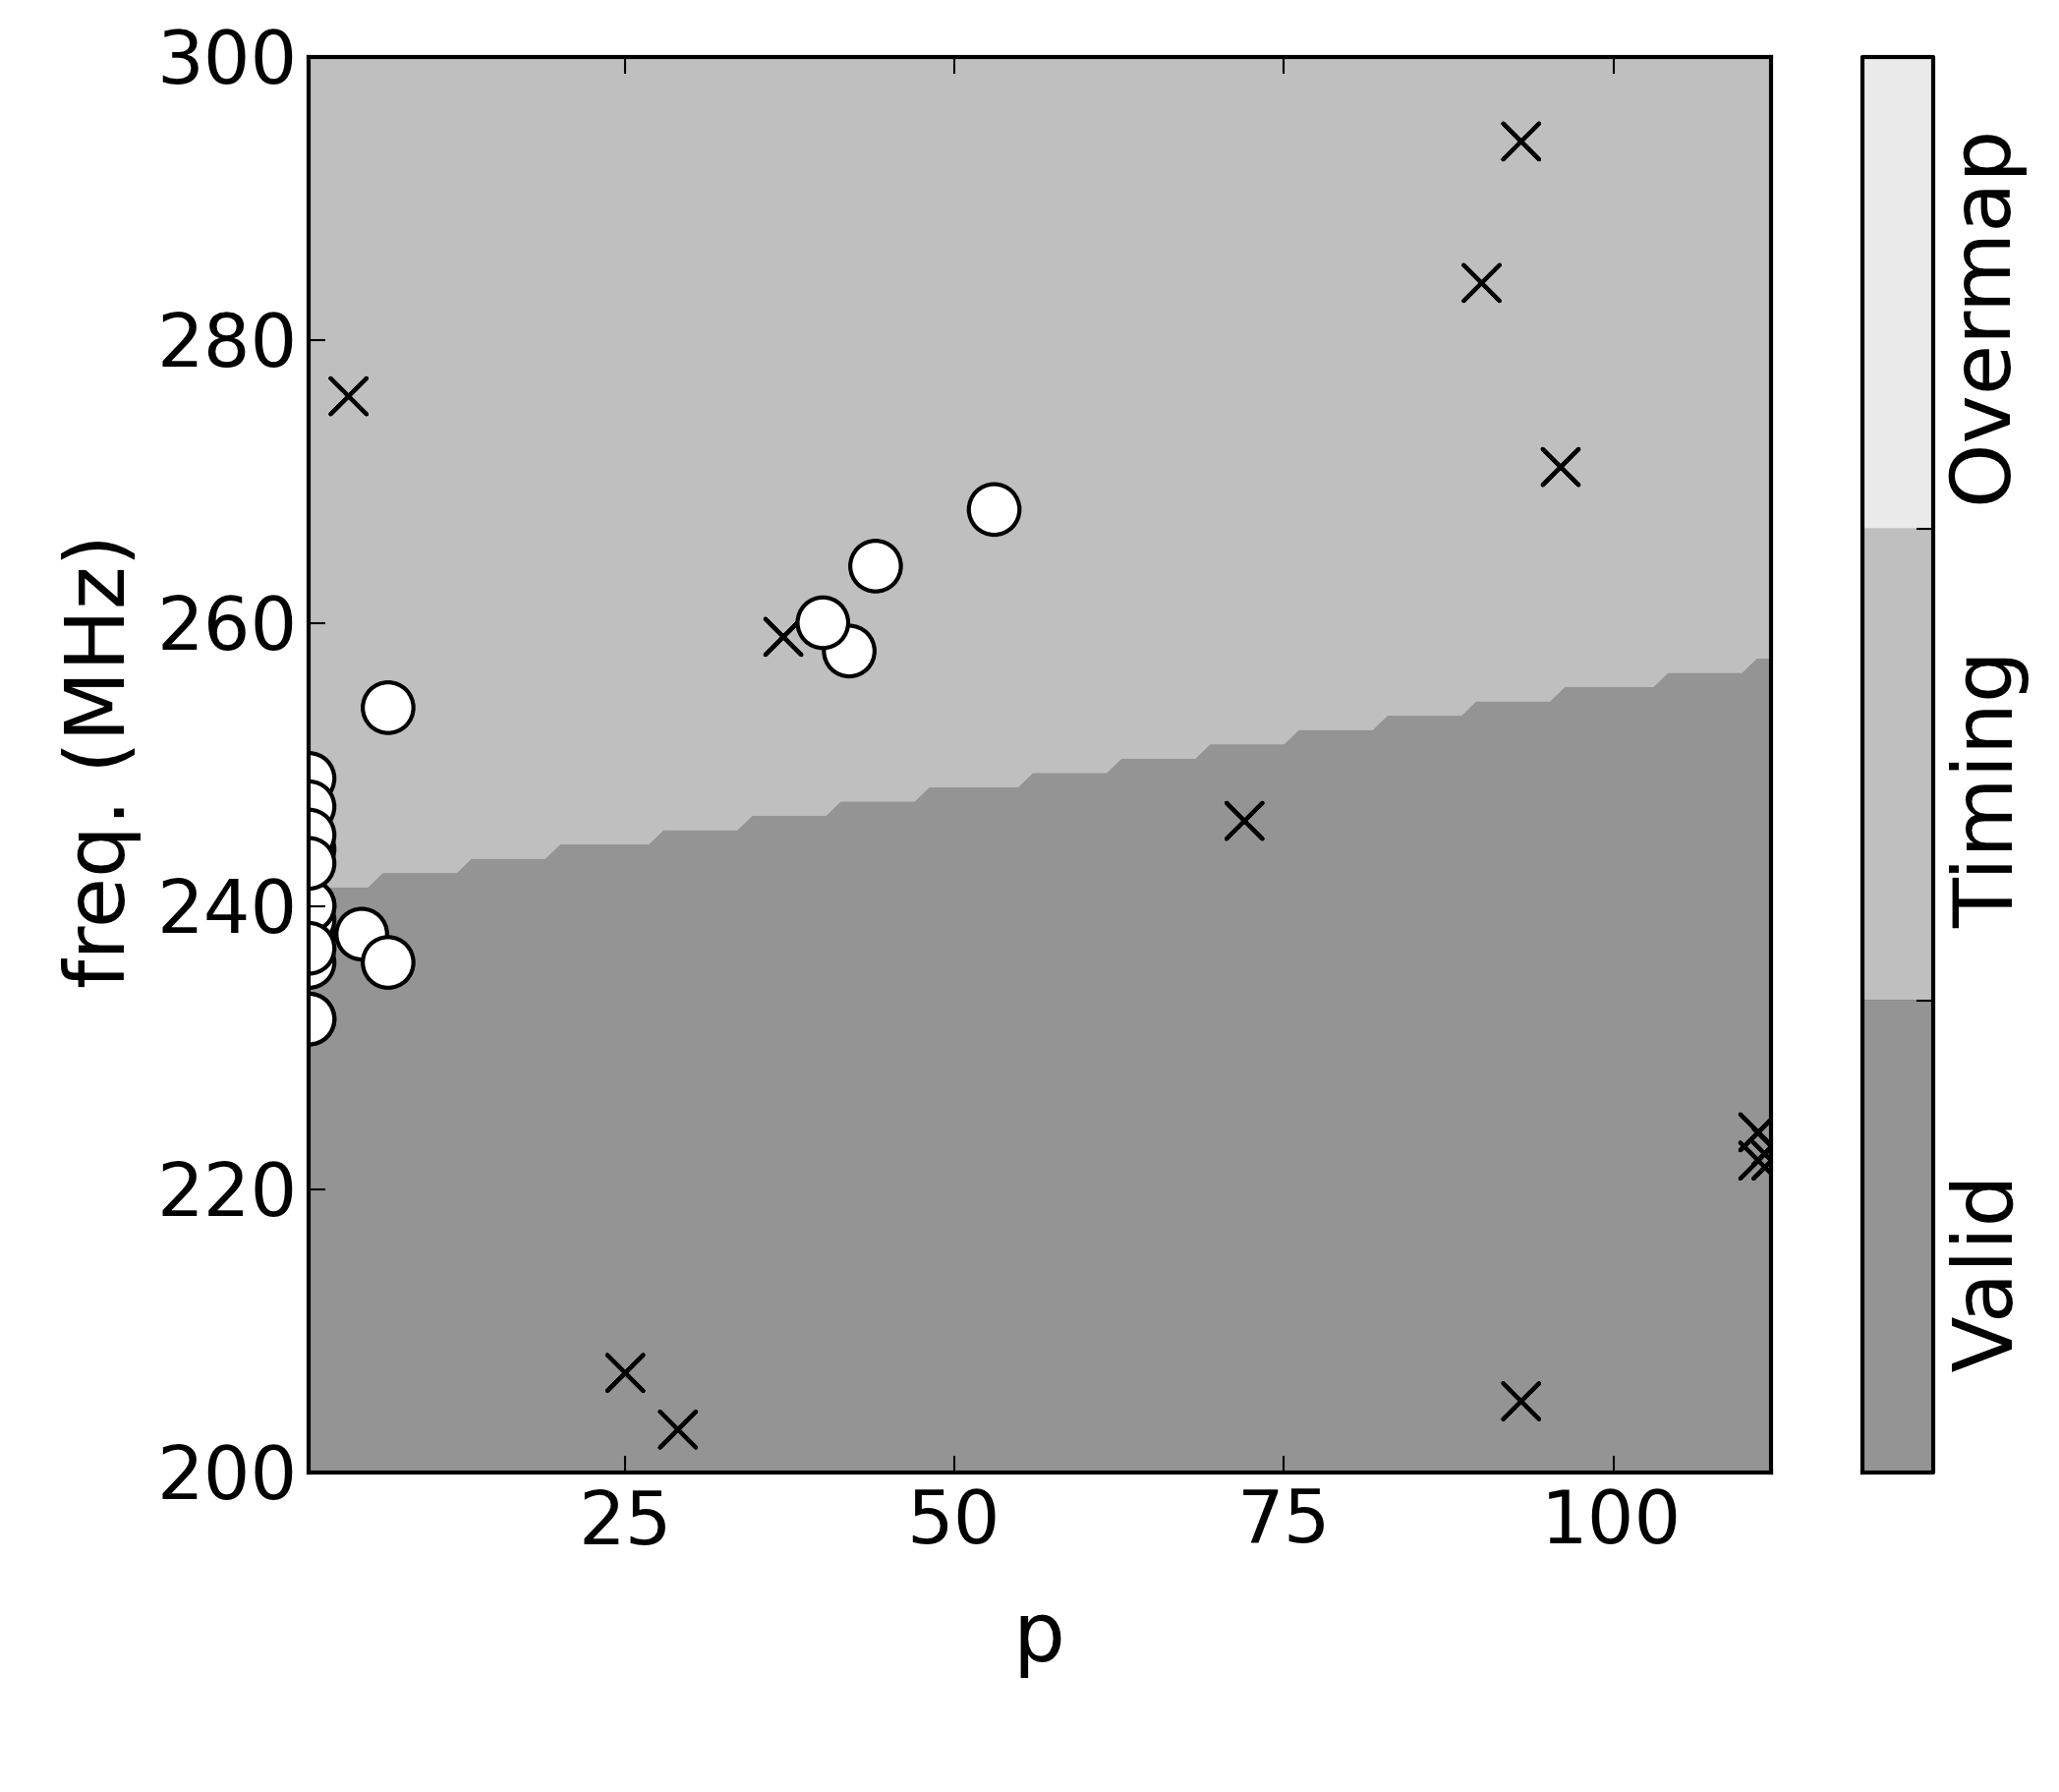
\includegraphics[width=\textwidth]{./figs/svm009_14.png}
        \end{subfigure}
        \begin{subfigure}{0.31\textwidth}
                \centering
                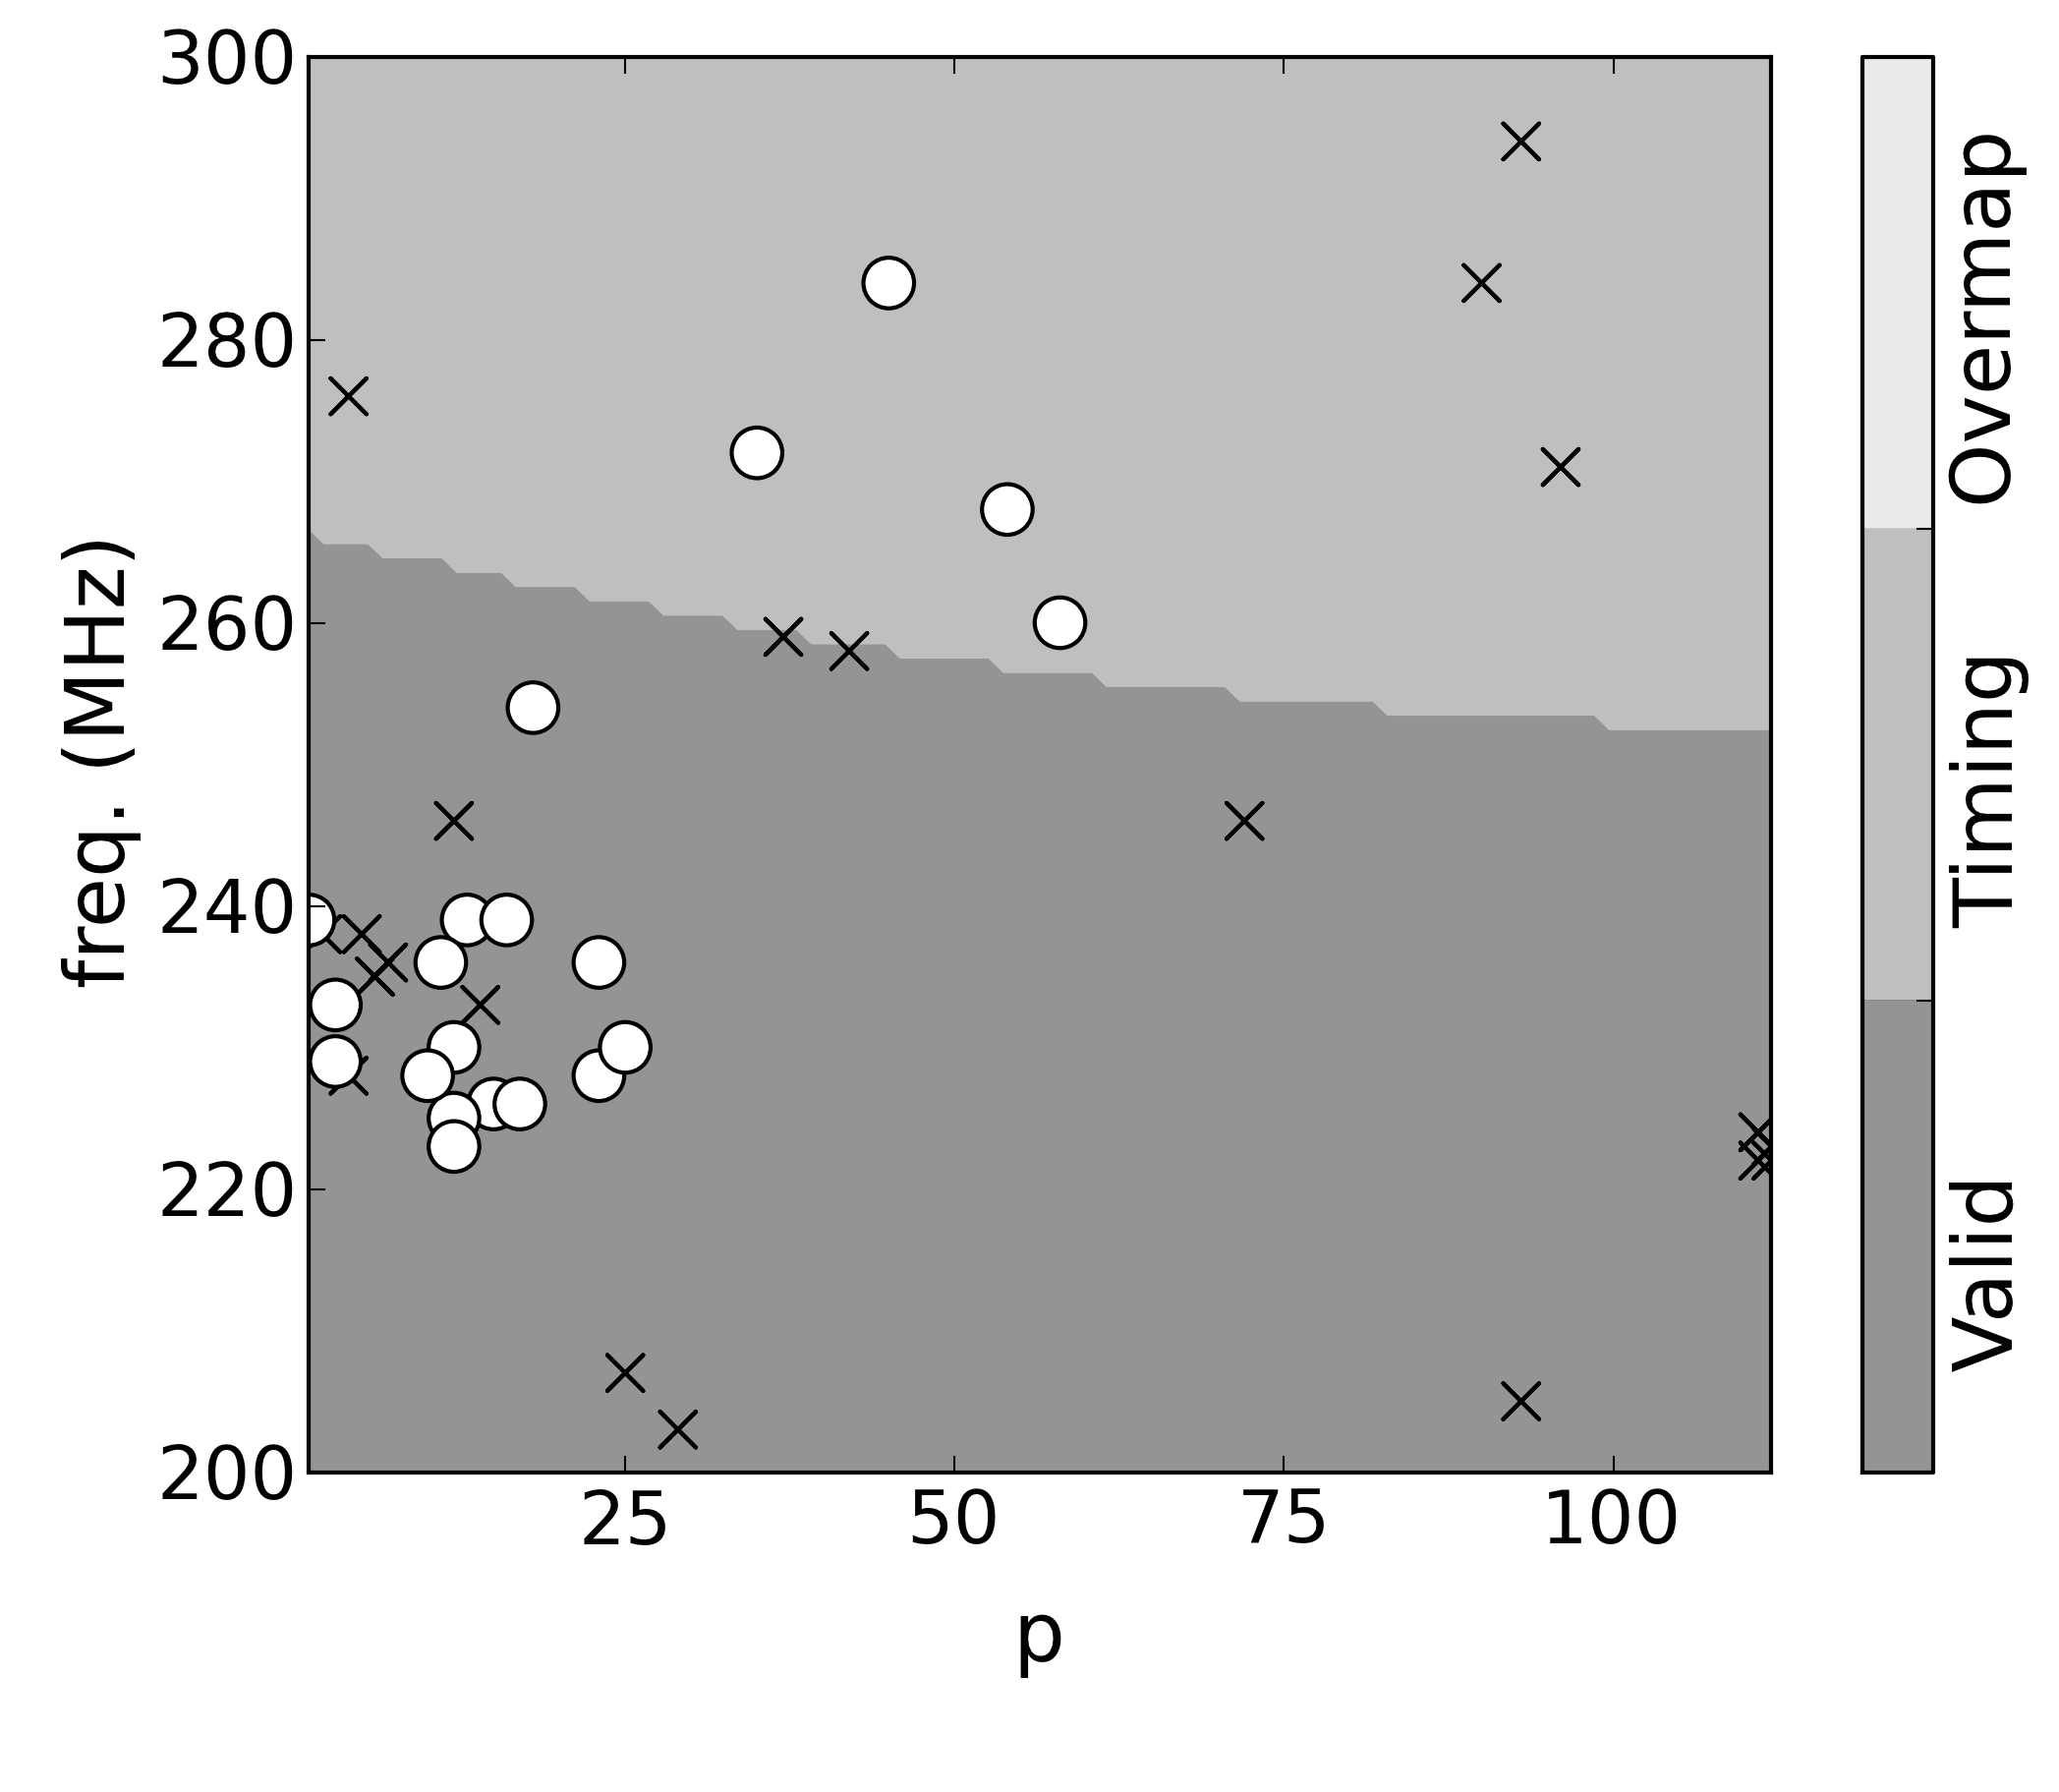
\includegraphics[width=\textwidth]{./figs/svm011_22.png}
        \end{subfigure}
        \caption{Optimization of $f$ ($\Phi_{config}$ = 300\,MB/s) after 13, 14 and 22 $f$ evaluations.}\label{fig:ansonsur}
\end{figure}


In Fig.~\ref{fig:fitness_2} we see how the \ac{svm} classifies a fraction of the
parameter space as $\mathcal{V}$ and how the surrogate model closely
matches the fitness function. We also see how particles collapse and
explore the optimal region $p\approx4$ for $\Phi_{config}$ = 5\,MB/s.
In Fig.~\ref{fig:fitness_1} we observe a similar situation but
for $\Phi_{config}$ = 300\,MB/s with the optimal region $p\approx20$.
Again, the surrogate model resembles the fitness function.
The collapse of particles is equivalent to the fine-tuning of the design parameters.
We present a visualization of the optimization in Fig.~\ref{fig:ansonsur}, each pair
of figures representing subsequent iterations. The top figures show the surrogate
model, while the bottom figures represent corresponding visualization of the design space and its classification.
During several initial iterations and $f$ evaluations, the particles (shown as white circles)
are misled by the surrogate model to explore $p\approx4$ region. In the last figure we
see particles guided by an improved surrogate model moving towards the optimum $p\approx20$ region.


%The \ac{alo} has not found any over-mapping examples. 

%\vspace{-2em}


%Benchmark design corresponds to step 1 in both approaches. In \cite{Anson2012Quad} $d_f=20$ is used to produce reference values and we evaluate a single benchmark portfolio rather then a range. As a reference design we use $m_{w}=53$ and $ d_{f}=32$.

%To measure the convergence rate the application terminates when the optimizer evaluates the design with highest throughput at specified precision ($\epsilon_{rms}$). 

%\vspace{-1.5em}

We use the reconfigurable radio benchmark to determine the impact of design space size on the convergence of the \ac{alo} algorithm. In Tab.~\ref{tab:radio1} we see a tendency of the number of $f$ evaluations to decrease along with the design space size. We trim design space by increasing the lower limit of admissible frequency $freq_{min}$. This shows that the designer should select a small parameter range as small design space improves \ac{alo} convergence. One outlier of $f=54$ in the case of $\Phi_{config}$=300\,MB/s and $freq_{min}$=200\,MHz can be explained with the overall small sample size. Manual optimization is replaced by \ac{alo}, which works with nearly no manual input but for the initial design space specification.

%\vspace{-1em}

%\vspace{-2em}


%
%As we only perform 10 test optimizations per setting we see that for $\Phi_{config}$=300\,MB/s and $freq_{min}$=200\,MHz \ac{alo} evaluated on average 54 fitness functions during each optimization, which breaks the general rule where smaller design improves convergence. Larger sample size should provide consistent results.


%In large scale designs the extra effort to extract marginally better performance might be justified. 

%table discussion


%  \begin{figure}
%     \centering
%\includegraphics[width=0.50\textwidth]{graphics/preeval.png}
%        \caption{\ac{alo} state after 13 $f$ evaluations. ($\Phi_{config}$ = 5\,MB/s)}     
%        \label{fig:5pre}
%  \end{figure}  
%  
%    \begin{figure}
%     \centering
%\includegraphics[width=0.50\textwidth]{graphics/posteval.png}
%        \caption{\ac{alo} state 13 $f$ evaluations later. ($\Phi_{config}$ = 5\,MB/s)}
%        \label{fig:5post}     
%  \end{figure}  
%  
%  
%  \begin{figure}
%     \centering
%\includegraphics[width=0.50\textwidth]{graphics/slow.png}
%        \caption{\ac{alo} state after 23 $f$ evaluations. ($\Phi_{config}$ = 300\,MB/s)}
%        \label{fig:300}     
%  \end{figure}  


\begin{table}
  \caption {Average number of $f$ evaluations - Reconfigurable radio optimization.}  
  \label{tab:radio1}
    \begin{center}
\begin{tabular}{c|cccc} 
\toprule 
 %&  \multicolumn{3}{c}{$\epsilon_{rms}$ } \\
	$\Phi_{config}$   & $freq_{min}$ & 150\,MHz & 200\,MHz & 220\,MHz\\\cline{2-5}  
	   5\,MB/s &  & 44 & 37 & 31 \\ 
       300\,MB/s & & 47 & 54 & 45 \\
\bottomrule 
\end{tabular} 
\end{center}
\end{table}

\subsection{Quadrature Method-based Application}
%\label{quadappbench}


%In \cite{Anson2012Quad} an analytical optimization scheme is proposed along with an associated algorithm that improves design throughput (integrations per second $\phi_{int}$) by varying the number representation in quadrature based applications. The tradeoff the designer faces is . 
%
% 

%relative error = 10^-3
In \cite{Anson2012Quad} the designer explores trade-off between accuracy and throughput in an application with three parameters. The first two parameters are mantissa width $m_{w}$ of the floating point operators and the number of computational cores $cores$. Larger number of $m_{w}$ bits increases computation accuracy, but limits the maximum number of $cores$ that can be implemented on the chip due to the increased size of the individual core. The third parameter is the density factor $d_{f}$ which specifies the density of quadratures used for integral estimation. It is a software parameter and is independent of the generated bitstream. Density factor $d_{f}$ increases computation time per integration while improving the accuracy of the results due to finer estimation of the integral. 

%\vspace*{-1em}


\begin{figure}
        \centering
        \begin{subfigure}[b]{0.31\textwidth}
                \centering
                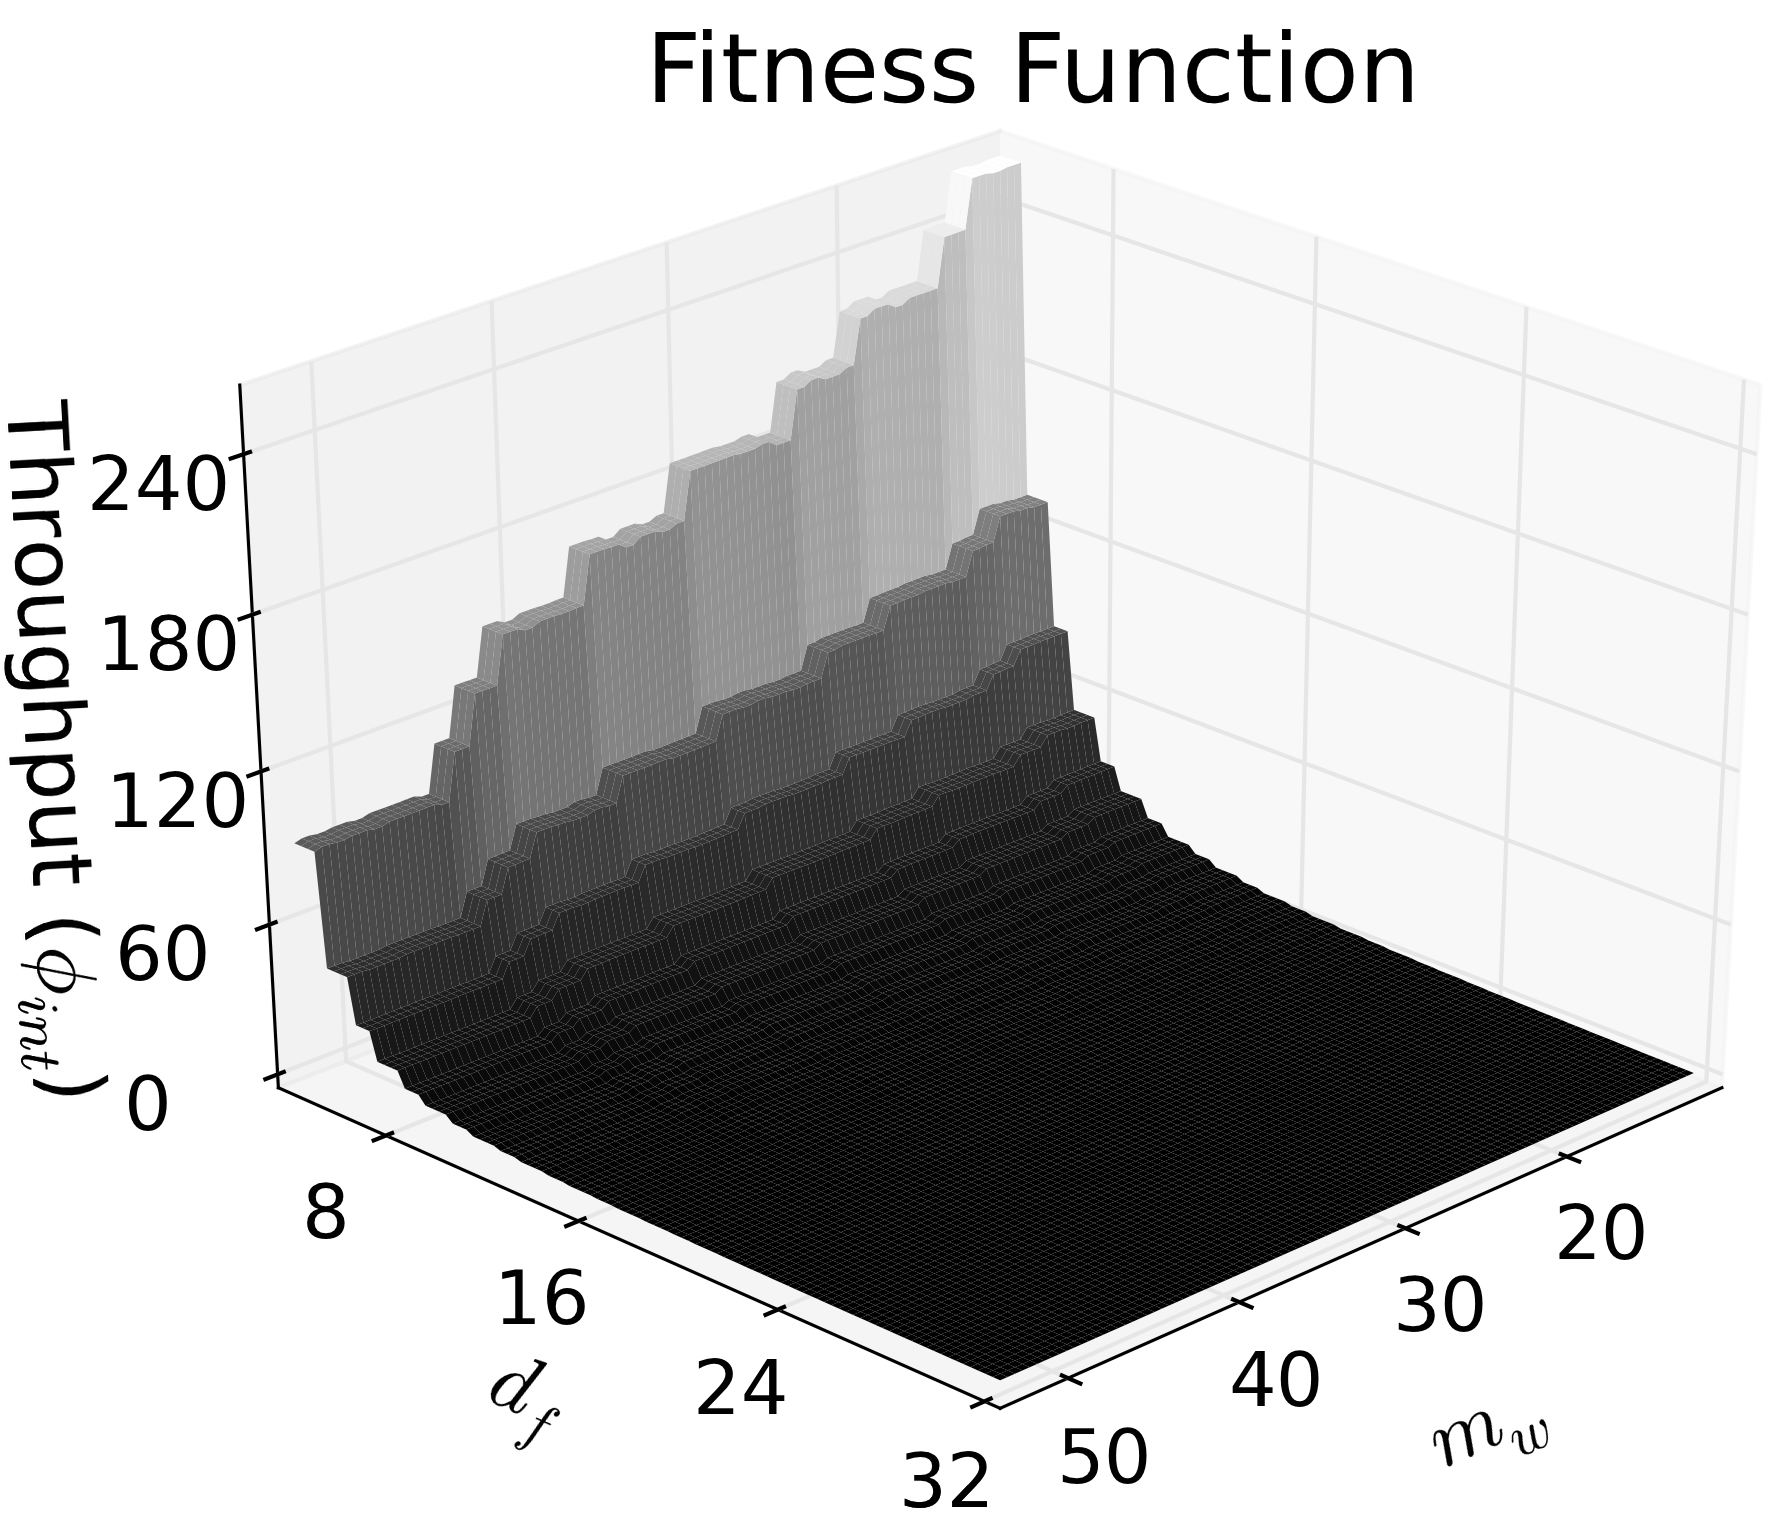
\includegraphics[width=\textwidth]{./figs/fitness_anson.png}
        \end{subfigure}
        \begin{subfigure}[b]{0.31\textwidth}
                \centering
                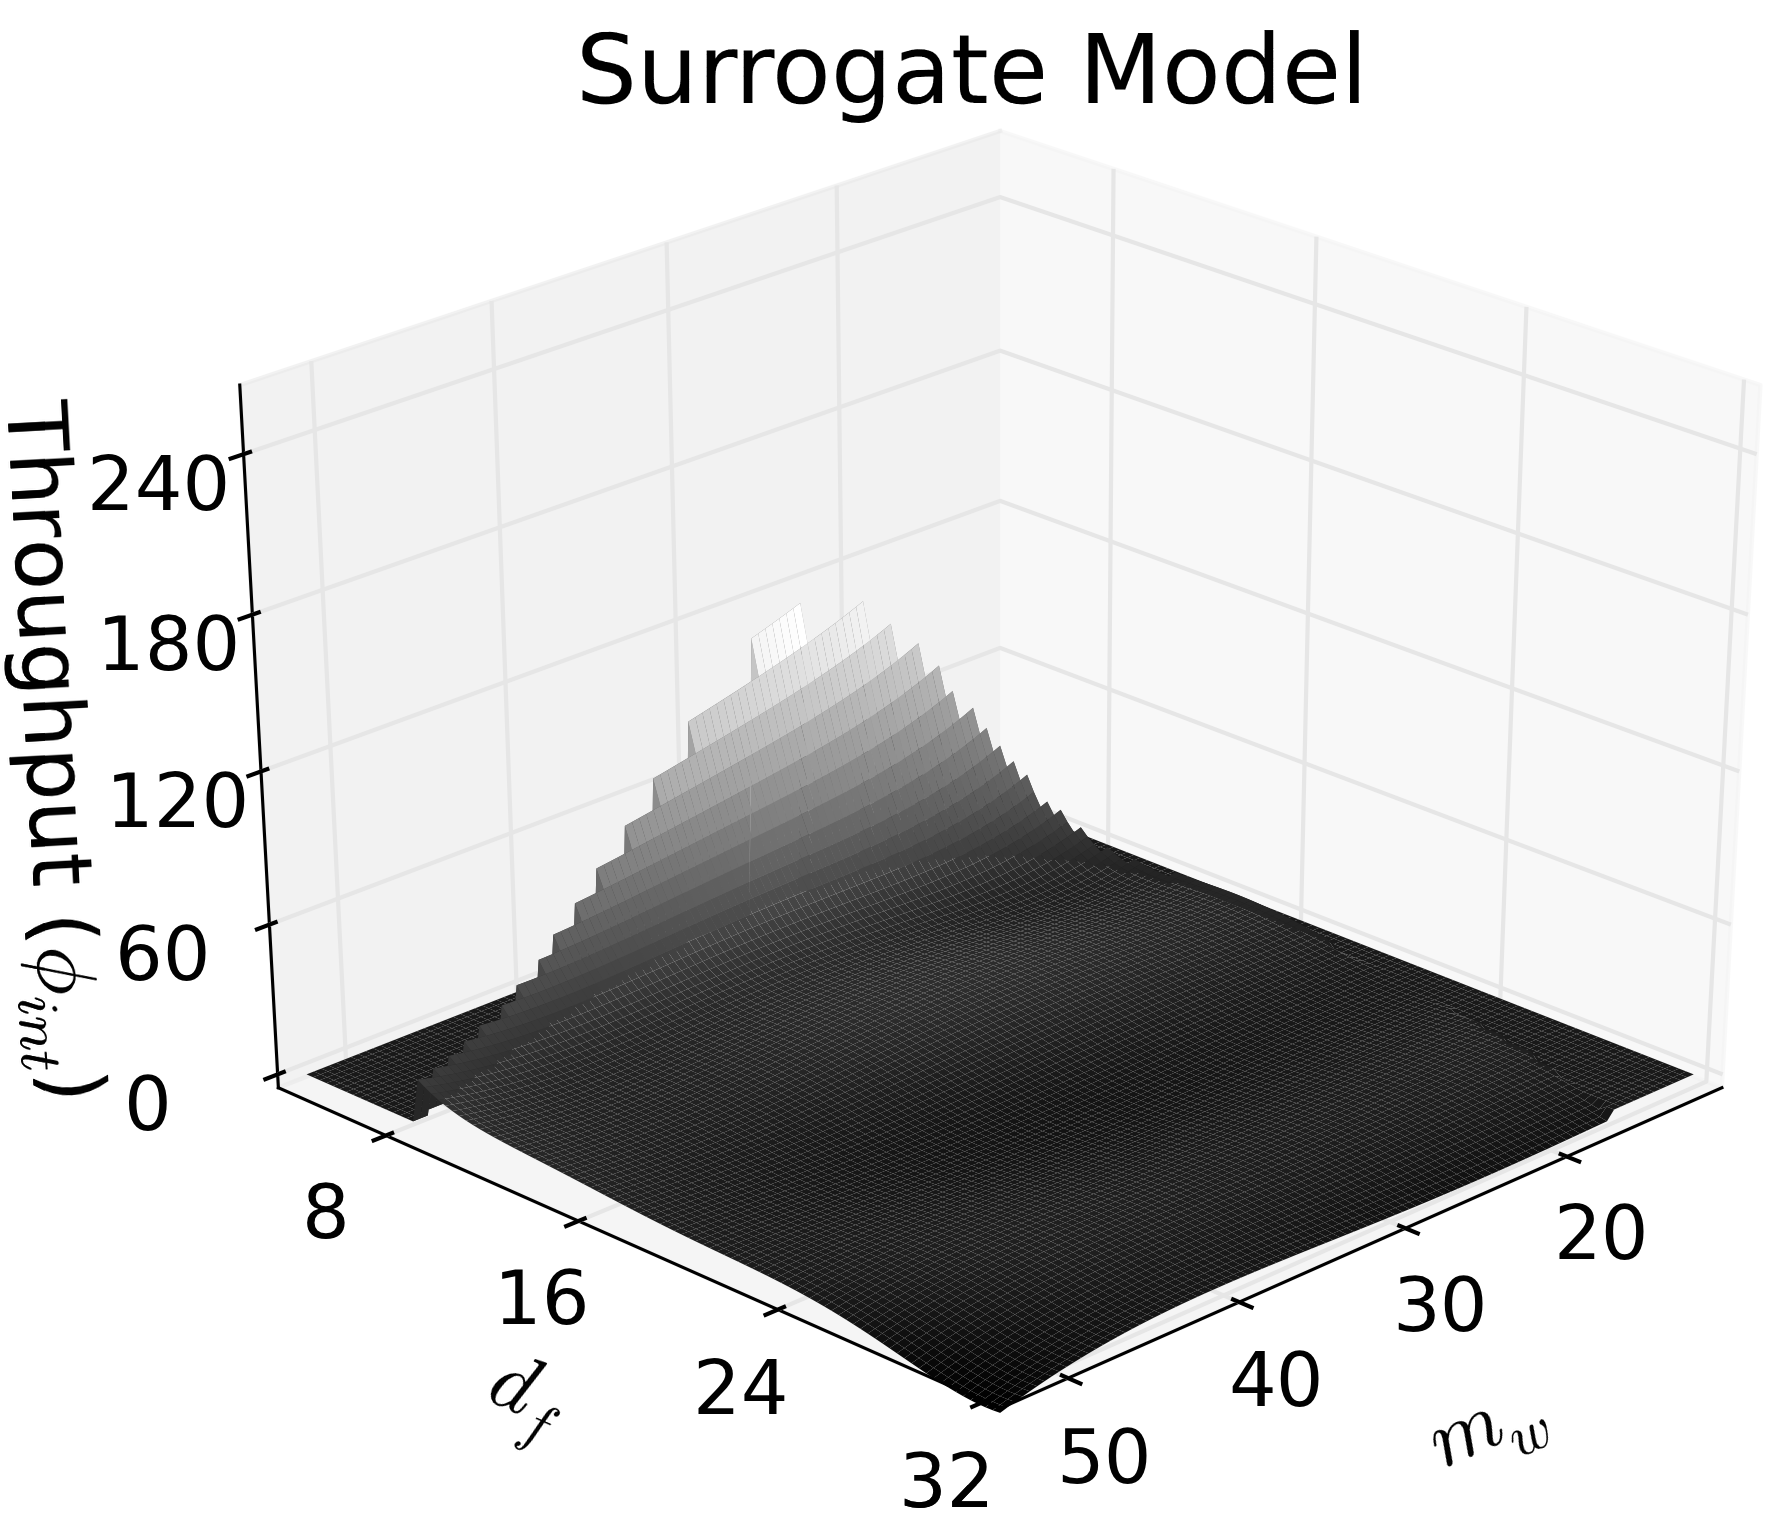
\includegraphics[width=\textwidth]{./figs/surmodel020_65_anson.png}
        \end{subfigure}
        \begin{subfigure}[b]{0.31\textwidth}
                \centering
                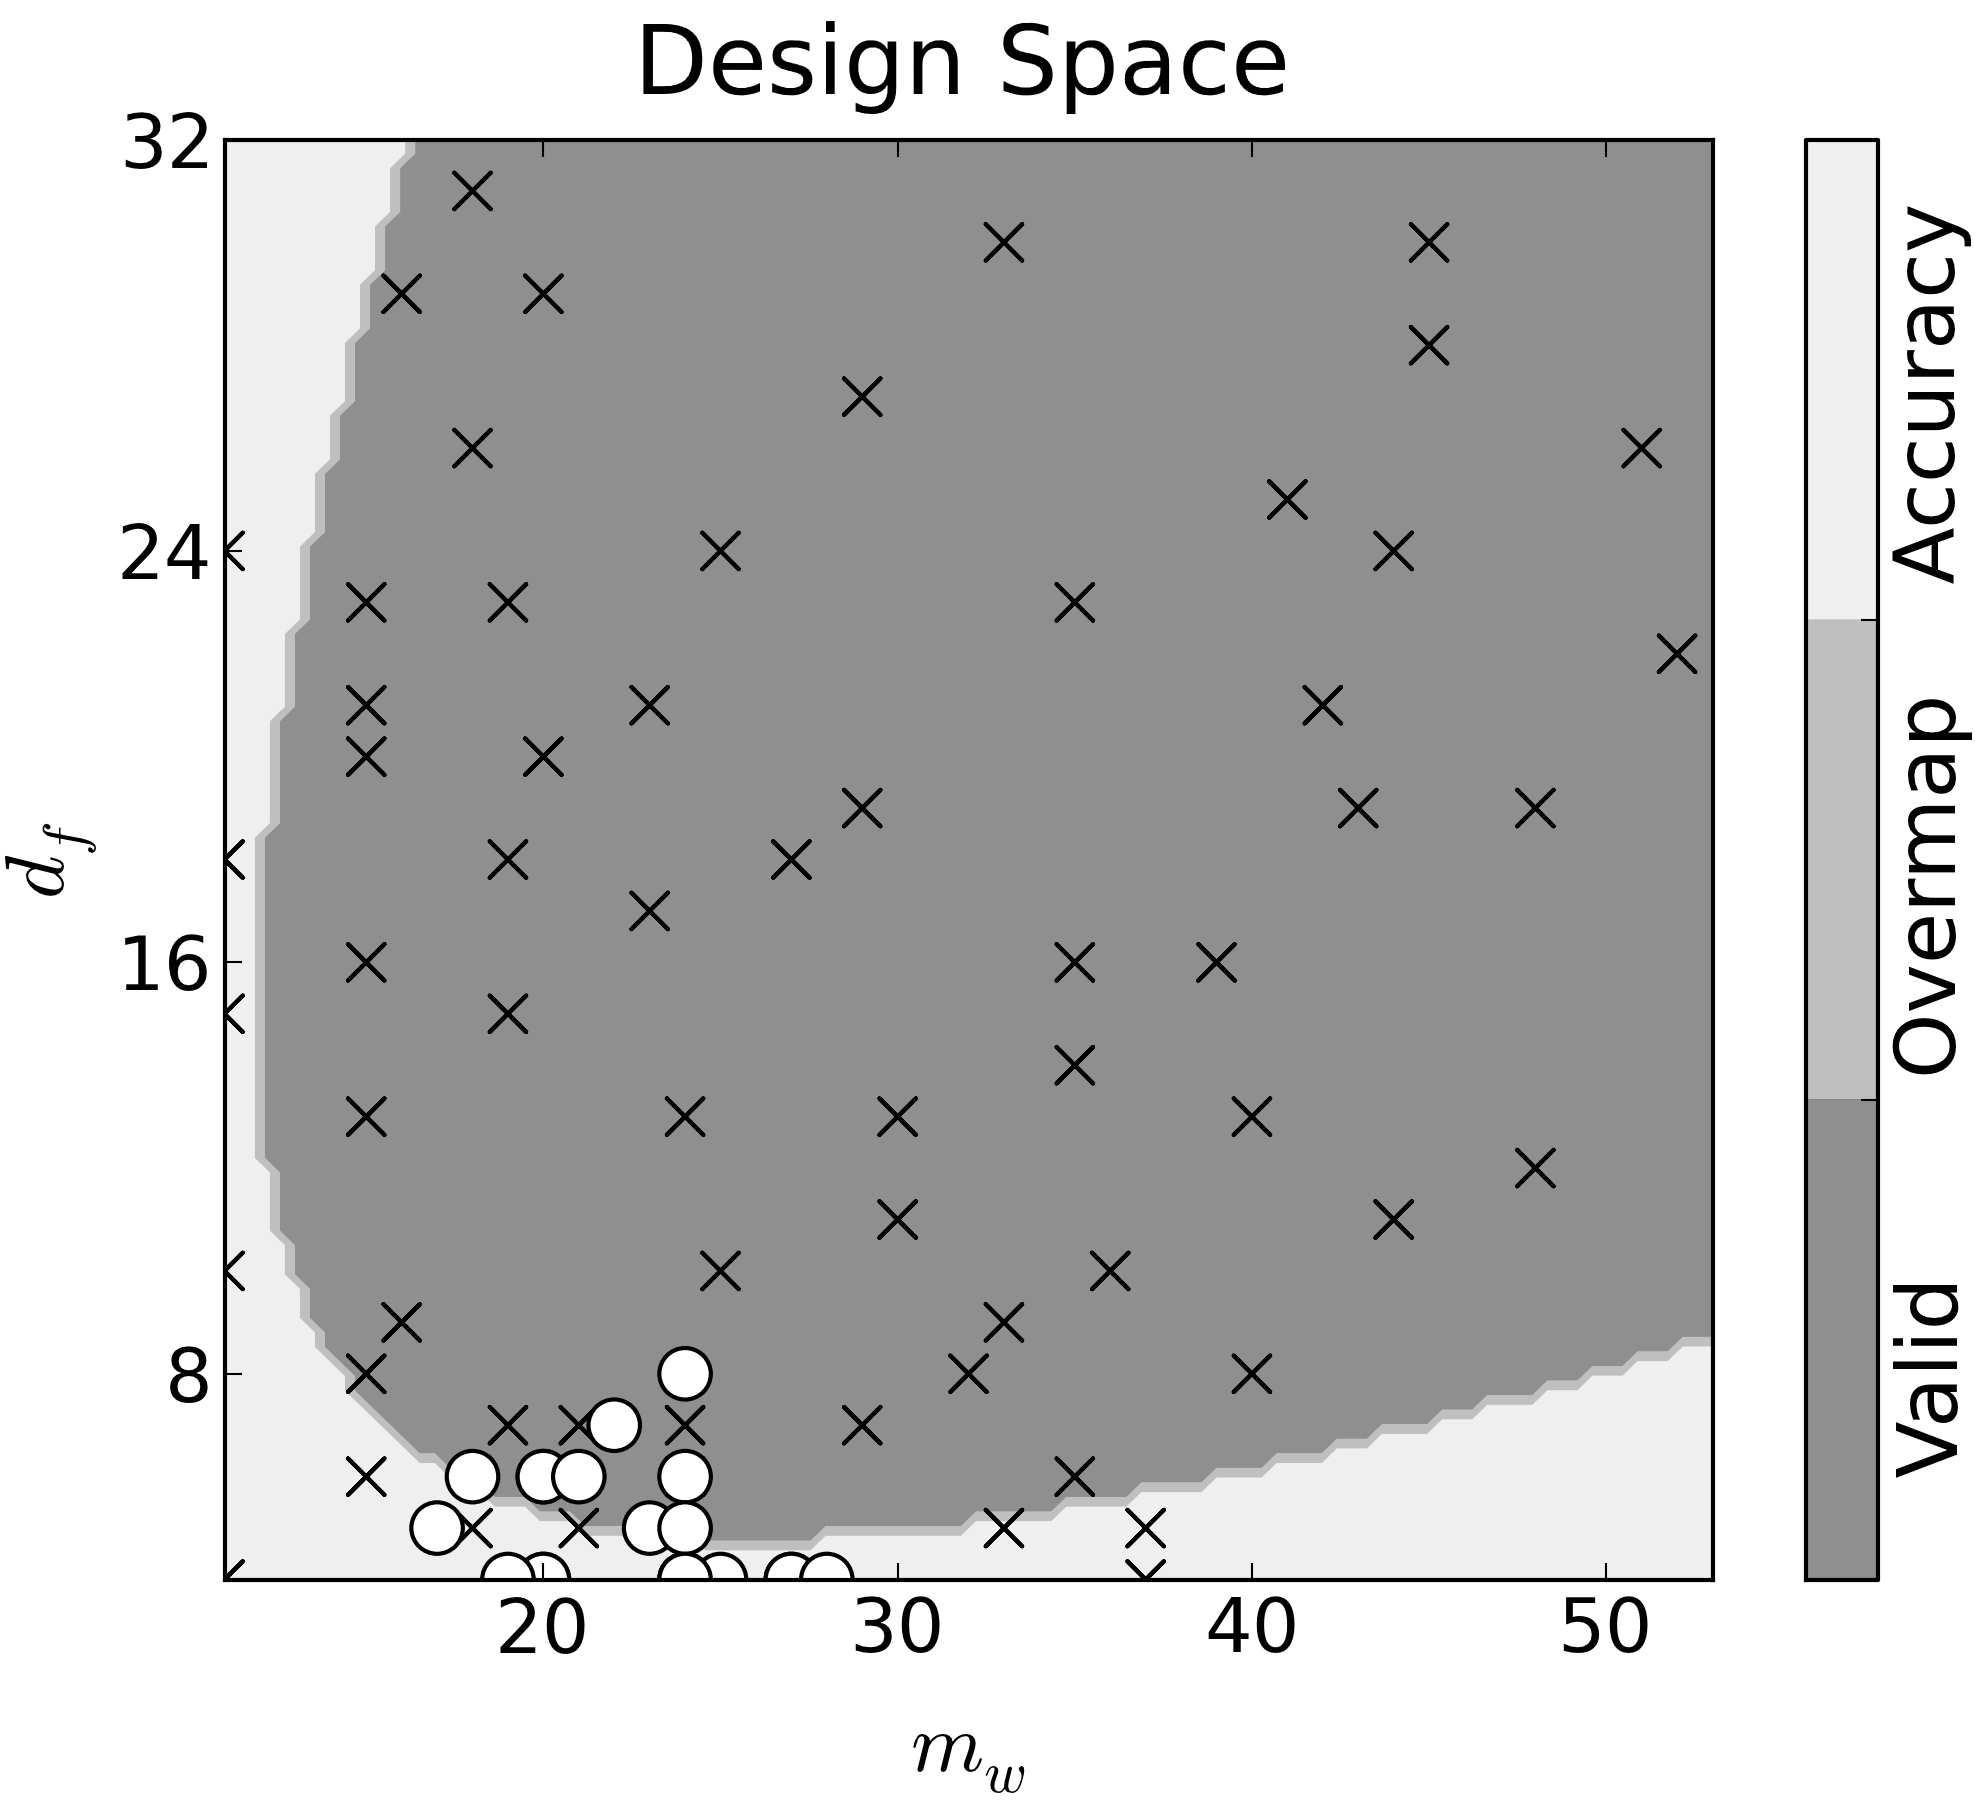
\includegraphics[width=\textwidth]{./figs/svm020_65_anson.png}
        \end{subfigure}
        \caption{Quadrature-based application $f$ and its surrogate model.}\label{fig:anson}
\end{figure}

%\vspace*{-1em}

The optimization goal is to find the design offering the highest throughput given a required minimum accuracy defined in terms of root mean square error $\epsilon_{rms}$. The error is defined with respect to results obtained by calculating a set of reference integrals at the highest possible precision. The \ac{alo} terminates when the globally optimal configuration for a given $\epsilon_{rms}$ is found. The $\mathcal{F}$ region contains the inaccurate result class, as these benchmark evaluations can be reused for regression. The design space $\mathcal{X}$ is defined as $m_w \times cores \times d_f $: $\{11-53\} \times \{1-16\} \times \{4-32\}$. We can explore the whole $\mathcal{X}$ in a three-dimensional scheme or we can reduce the three-dimensional problem into two dimensions using an analytical resource usage estimation model. Resource usage is linearly related to $cores$, and after generating a single $core$ bitstream we can create a simple analytical resource model which reduces the parameter space to two dimensions. Density factor $d_{f}$ is a software parameter while $m_w$ and $cores$ affect the bitstream. Varying $d_f$ only involves software execution, as long as a bitstream for the given $m_w$ is already generated. If we evaluate a design with $m_w$ (or $m_w$, $cores$) that has not been evaluated before, we generate a new bitstream.

 We present a visualization of the two-dimensional optimization in Fig.~\ref{fig:anson}, where the $\epsilon_{rms}$ limit is set to a value of 0.1. The bottom-left corner of $\mathcal{V}$ contains the global optimum which is difficult to determine without additional benchmark evaluations, as the maximum number of possible $cores$ and therefore throughput is limited by \ac{fpga} resources and as a result is chip dependent. Regions of space with low $d_f$ or $m_w$ are correctly predicted to offer low accuracy (light gray area). 
 
\begin{table}
  \caption {Average number of $f$ evaluations - Quadrature application optimization.}  
  \label{tab:anson}
    \begin{center} 
\begin{tabular}{c|cccc} 
\toprule 
 %&  \multicolumn{3}{c}{$\epsilon_{rms}$ } \\
	 $cores$  & $\epsilon_{rms}$ & 0.1 & 0.01 & 0.001 \\\cline{2-5}  
	  three-dimensional &  & 138 & 67 & 47 \\ 
       two-dimensional & & 71 & 43 & 28 \\
\bottomrule 
\end{tabular} 
\end{center}
\end{table}


To measure the algorithms convergence the \ac{alo} terminates when the design with the highest throughput at the specified precision is found. The number of required $f$ evaluations is shown in Tab. \ref{tab:anson}. The previously suggested optimization scheme \cite{Anson2012Quad} involves generating bitstreams for the full $m_w$ range. Using our \ac{alo} combined with the analytical resource model, we reduce the number of bitstream generations as we avoid exploring $cores$ and thus decrease the design space. Around 20-50\% of $f$ evaluations involve bitstream generation. The number has a high variance between individual runs as the swarm either skips undesirable configurations or thoroughly explore the whole design space.

The optimization scheme presented in \cite{Anson2012Quad} involves generating all possible bitstreams with $cores=1$, and a binary search of the $d_f$ values. Once the optimal ($d_f,m_w$) tuple is found, the number of $cores$ can be determined. It also requires the generation of bitstreams for all $m_w$ resulting in 53-11=42 distinct bitstreams. Furthermore, the number of bitstreams is nearly doubled since after the first generation, usually a second bitstream generation follows to adjust $cores$. Binary search is performed on the $d_f$ range of 32-4=28 distinct values per bitstream, which yields on average $2 \times \lceil\log_2 \left( 28 \right)\rceil= 10$ benchmark evaluations per bitstream.


In comparison the \ac{alo} performance can be measured both in terms of $f$ evaluations and bitstream generations. Using the optimization approach from \cite{Anson2012Quad} we perform a binary search on $d_f$ range for all $m_w$ values resulting on average $10 \times 42 = 420$ $f$ evaluations regardless of the $\epsilon_{rms}$ limit. As presented in Tab.~\ref{tab:anson} for $\epsilon_{rms}=0.1$ the \ac{alo} requires 75 evaluations (85 \% less) in the two-dimensional scheme and 138 (67 \% less) in the three-dimensional scheme. The number becomes more favorable for the \ac{alo} when $\epsilon_{rms}$ is reduced as $\mathcal{V}$ is decreased and the \ac{alo} needs to explore a smaller area, while average number of $f$ evaluations in their optimization approach stays constant. Not all $f$ evaluations involve bitstream generations: for $\epsilon_{rms}=0.1$, 50\% of $f$ evaluations involve two bitstream generations resulting in 71 bitstreams compared to 82 bitstreams in \cite{Anson2012Quad}. In the three-dimensional scheme, \ac{alo} further decreases number of bitstream generations, to an average of 69. Our automated approach clearly outperforms manual design both in terms of $f$ evaluations and bitstream generations, although in the second case the results are less dominant. 

%In three-dimensional case only single bitstream is evaluated per configuration. 






%We generate a single core bitstream and depending on $U_{slice}$ (and $m_w$ indirectly) generate a second multi-core bitstream. 

% \begin{table}
%  \caption {Parameters.}  
%    \begin{center}
%\begin{tabular}{p{3.5cm} p{3.5cm}}
%\hline Parameter & Value Range \\ 
%\hline $m_{w}$ &  11-53\\ 
%       $d_{f}$ &  4-32\\ 
%       $cores$ & 1-16 \\
%\hline 
%\end{tabular} 
%\end{center}
%\end{table}

%Although the model is clearly defined it is application specific, and non-obvious. Following our approach one would simply design parameterizable kernel(s) and a benchmark, and run the optimizer to obtain the optimal set. Following \cite{Anson2012Quad} one has to understand the application, and follow the more tedious approach. Furthermore if the underlying algorithm changes a new optimization scheme would have to be devised - we offload the user by allowing him to be totally ignorant about analytical optimization.


%\begin{figure}
%        \centering
%
%        \caption{\ac{svm} state after 19, 63 and 128 $f$ evaluations}\label{fig:ansonsvm}
%\end{figure}


%As shown before, the proposed \ac{alo} approach involves fewer bit stream generations when compared with the traditional approach, up to a reduction of 85\% in the case of a financial benchmark based on the quadrature algorithm. Moreover, since our \ac{alo} approach adopts a generic algorithm (Algorithm 1), it often takes significantly less time to use it for a given application, than the traditional approach which would involve creating multiple application-specific algorithms for parameter optimization, one for each application.

%The results indicate that higher the $\epsilon_{rms}$ limit the lower the number of $f$ evaluations. This is the case as $\mathcal{X}$ is being restricted using \ac{svm}. 


\section{Conclusions and Future Work}

We have proposed \ac{alo}, a novel tool which can determine optimized parameter configuration of a reconfigurable \ac{fpga} design. The \ac{alo} can offer superior performance, while reducing effort on analysis and application-specific tool development. The main advantage of using the \ac{alo} is a shift from manual optimization to automatic computation. The \ac{alo} requires multiple benchmarks for further evaluation, and there are many opportunities for future work; an example is the development of new surrogate models that would allow the reduction of required benchmark samples and efficiently address high dimensional examples. There are numerous cases where level of parallelism, timing and other parameters span tens of dimensions and would benefit from an effective  automated approach.

\subsubsection*{Acknowledgements}
This work is supported by the European Union Seventh Framework Programme under grant agreement number 248976, 257906, 287804 and 318521, by UK EPSRC, by Maxeler University Programme, and by Xilinx.
 
\bibliographystyle{IEEEtran}
\bibliography{Paper32}

%
%%---------------------------------------------------------------------------%%

\end{document}


